%
% LaTeX-Rahmen für Arbeiten am Lehrstuhl Hegering
%
% Nils gentschen Felde, 01/2006
%
% basierend auf Arbeiten von Helmut Reiser, Boris Gruschke,
% Stephen Heilbronner und Harald Rölle
%

\documentclass[a4paper,10pt,twoside,DIV14,BCOR14mm]{scrreprt} 


% !!!!
% !!!! Auswählen der Sprache
% !!!!
\newif\ifLANGDE\LANGDEtrue\newif\ifLANGEN\LANGENfalse   % aktivieren für Deutsch
% \newif\ifLANGEN\LANGENtrue\newif\ifLANGDE\LANGDEfalse   % aktivieren für Englisch


% !!!!
% !!!! Auswählen der Uni
% !!!!
%\newif\ifTUM\TUMtrue\newif\ifLMU\LMUfalse   % aktivieren für TUM
\newif\ifLMU\LMUtrue\newif\ifTUM\TUMfalse   % aktivieren für LMU



% !!!!
% !!!! Auswählen des Typs der Ausarbeitung
% !!!!
%\newcommand{\typeOfThesis}[0]{Diplomarbeit}
\newcommand{\typeOfThesis}[0]{Fortgeschrittenenpraktikum}
%\newcommand{\typeOfThesis}[0]{SEP}
%\newcommand{\typeOfThesis}[0]{Studienarbeit}


% !!!!
% !!!! Titel der Arbeit
% !!!!
\newcommand{\titleOfThesisOne}[0]{Virtuelle Systeme Praktium - Gruppe 1}
\newcommand{\titleOfThesisTwo}[0]{}
\newcommand{\titleOfThesisThree}[0]{}


% !!!!
% !!!! Verfasser der Arbeit
% !!!!
\newcommand{\authorOfThesis}[0]{Vorname Nachname}


% !!!!
% !!!! Aufgabensteller
% !!!!
\newcommand{\aufgabensteller}[0]{Prof. Dr. Dieter Kranzlm\"{u}ller}
%\newcommand{\aufgabensteller}[0]{Prof. Dr. Heinz-Gerd Hegering}
%\newcommand{\aufgabensteller}[0]{Prof. Dr. Claudia Linnhoff-Popien}


% !!!!
% !!!! Betreuer
% !!!!
\newcommand{\betreuerOne}[0]{Vorname Name vom ersten Betreuer}
\newcommand{\betreuerTwo}[0]{Vorname Name vom zweiten Betreuer}
\newcommand{\betreuerThree}[0]{Vorname Name vom dritten Betreuer}


% !!!!
% !!!! Abgabedatum
% !!!!
\newcommand{\abgabeTagZahl}[0]{14}
\newcommand{\abgabeMonatText}[0]{Juli}
\newcommand{\abgabeJahrZahl}[0]{2006}


% !!!!
% !!!! Bibtex files auswählen
% !!!!
% !!!! Variante nur mit lokalen bibfiles (läuft überall)
% !!!!
\newcommand{\bibfiles}[0]{bibfile1}
% !!!!
% !!!! Variante inklusive der MNM bibfiles (läuft nur am Lehrstuhl)
% !!!!
%\newcommand{\bibfiles}[0]{bibfile1,articles,rfcs,internet-drafts,publikationen,diplomarbeiten,dissertationen,fopras,projekte,books,ref,std,in-proceedings,proceedings,ietf-wgs,omg}


% !!!!
% !!!! Auswählen ob Abkürzungsverzeichnis oder Glossar
% !!!!  Wenn man ein Glossar benutzt, dann sollten Abkürzungen 
% !!!!  einfach ins Glossar mitaufgenommen werden.
% !!!!
\newif\ifISGLOSS\ISGLOSSfalse   % aktivieren für Abkürzungsverzeichnis
%\newif\ifISGLOSS\ISGLOSStrue    % aktivieren für Glossar


%=============================================================================================
% Einbinden der MNM-Definitionen
%=============================================================================================

%
% LaTeX-Rahmen für Arbeiten am Lehrstuhl Hegering
%
% Harald Roelle, 2001,2002
%
% basierend auf Arbeiten von Helmut Reiser, Boris Gruschke und Stephen Heilbronner
%


%=============================================================================================
% Allgemeine Schalter bezueglich des Ausgabeformats
%  MUSS MAN I. A.   N I C H T   ANFASSEN
%=============================================================================================

%
% Check for pdftex
%
%\newif\ifpdf
%\ifx\pdfoutput\undefined
%  \pdffalse % we are not running PDFLaTeX
%\else
%  \pdfoutput=1 % we are running PDFLaTeX
%  \pdftrue
%\fi
\usepackage{ifpdf}


%=============================================================================================
% Einbinden von Packages
%=============================================================================================

% muss ganz am Anfang stehen!
\ifLANGDE%
  \usepackage[british,german]{babel} % => german ist Default zu Beginn (stimmt wirklich!)
  \usepackage{german}        % (neue) deutsche Silbentrennung, ...
  \usepackage{bibgerm}       % deutsche Literaturverzeichnisse
\fi%
\ifLANGEN%
  \usepackage[german,english]{babel} % => english ist Default zu Beginn (stimmt wirklich!)
\fi%

% \usepackage{a4wide}        % weniger Rand  % koenig
\usepackage{url}           % URL's (z.B. in Literatur) schöner formatieren
% \usepackage{tocbibind}     % Literaturverzeichnis erscheint im Inhaltsverz.
\usepackage{supertabular}  % Besonders flexible und grosse Tabellen
\usepackage{makeidx}       % unterstuetzt \makeindex
\usepackage{picins}        % (kleine) Bilder vom Text umfliessen lassen (neu)
% \usepackage{mdwlist}       % für (engere) itemize*-Umgebungen  % koenig
\usepackage{multicol}
% \usepackage{rotating}  % koenig
% \usepackage{epsfig}    % koenig
\usepackage{graphicx}
\usepackage{graphics}
\usepackage{wrapfig}
\usepackage{ifthen}

\usepackage{tikz}
\usepackage{pgfplots}
\usepgfplotslibrary{units}

\usepackage{alltt}

%\usepackage{tabularx} % für Tabellen automagischer Feldbreiten berechnung
%\usepackage{multirow} % für Tabellenfelder, die sich über mehrere Zeilen erstrecken
%\usepackage{subfigure} % um mehrere Abbildungen in einer figure-Umgebung zu strukturieren
%\usepackage{paralist} % für kompakte und nutzerdefinierte itemize und enumerate umgebungen

\ifLANGDE%
  \usepackage[german]{nomencl}       % Abkürzungsverzeichnis
  \ifISGLOSS%
    \renewcommand{\nomname}{Glossar}%
  \else%
    \renewcommand{\nomname}{Abk\"{u}rzungsverzeichnis}%
  \fi%
\fi%
\ifLANGEN%
  \usepackage[english,compatible]{nomencl}       % Abkürzungsverzeichnis
  \ifISGLOSS%
    \renewcommand{\nomname}{Glossary}%
  \else%
    \renewcommand{\nomname}{List of Abbreviations}
  \fi%
\fi%
\renewcommand{\nomlabel}[1]{\textbf{#1}\hfil}%
 
\usepackage{parskip}


%
% Times als Font einstellen
%
\usepackage{rawfonts}
\usepackage{times}


%
% Umlaute direkt im Quellcode
%
% \usepackage[iso]{umlaute}  % koenig

\usepackage[utf8]{inputenc}


%
% Ermöglicht den Pretty-Print der Programmcodes
%
\usepackage{listings}
%\usepackage[breaklines]{listings}
%
% Standards für die Ausgabe der Pretty-Prints !!! SMALL !!!
%
 \lstset{basicstyle=\small\ttfamily, keywordstyle=\bfseries,
  commentstyle=\color{blue}, stringstyle=\itshape,
  extendedchars=true}
% XXXXXXXXXXXXXXXXXXXXXX
%  labelstyle=\tiny\ttfamily, labelstep=2, labelsep=5pt, extendedchars=true}
% numberstyle=\tiny\ttfamily, stepnumber=2, numbersep=5pt, extendedchars=true}


%
% Easy way changing title/section/... appearence
%
\usepackage{titlesec}


%
% muss an dieser Stelle stehen
%
%\usepackage{html}
\usepackage{hyperref}


%
% PDF-Spezifische Angaben
%
\ifpdf
  \pdfcompresslevel=9
  %\usepackage{thumbpdf}  % koenig
  \hypersetup{ a4paper=true,
               plainpages=false,
               pdftex=true,
               hyperindex=true,
               bookmarks=true,
               bookmarksopen=true,
               bookmarksnumbered=true,
               pdfauthor={\authorOfThesis},
               pdftitle={\titleOfThesisOne \titleOfThesisTwo \titleOfThesisThree}
             }
\fi

%
% Rudimentäre Kommentar-Makros
%
\usepackage{color}

\definecolor{fixmecolor}{rgb}{1.0,0.4,0.4}
\definecolor{todocolor}{rgb}{0.4,1.0,0.4}
\definecolor{notecolor}{rgb}{0.4,0.4,1.0}

\newcommand{\fixme}[1]{\textcolor{fixmecolor}{[FIXME: #1]}}
\newcommand{\todo}[1]{\textcolor{todocolor}{[TODO: #1]}}
\newcommand{\note}[1]{\textcolor{notecolor}{[NOTE: #1]}}

%Kommentare für finalen Build ausschalten:
%\newcommand{\fixme}[1]{}
%\newcommand{\todo}[1]{}
%\newcommand{\note}[1]{}

%
% In geralpha-mnm-0.2.bst wird \mnmbiburl als Makro zum Erstellen der URL Links benutzt
% Das hier benutzte \refHTML funltioniert in tex, pdf und html
%
\newcommand{\mnmbiburl}[2]{\refHTML{#1}{#2}}


%=============================================================================================
% Einige Makros
%=============================================================================================

\newcommand{\product}[2][X]{%
  \if#1X%
  \else%
    \index{#1#2}%
  \fi%
  \textsl{#2}%
}

\newcommand{\vendor}[2][X]{%
  \if#1X%
  \else%
    \index{#1#2}%
  \fi%
  \textsf{#2}%
}

\newcommand{\code}[2][X]{%
  \if#1X%
  \else%
    \index{#1#2}%
  \fi%
  \texttt{#2}%
}

\newcommand{\filepath}[2][X]{%
  \if#1X%
  \else%
    \index{#1#2}%
  \fi%
  \texttt{#2}%
}

\newcommand{\texturl}[2][X]{%
  \if#1X%
  \else%
    \index{#1#2}%
  \fi%
  \texttt{#2}%
}


%=============================================================================================
%
% Abkürzungsverzeichnis und Glossar
%

\newcommand{\newAbbrev}[4][X]{%
  \if#1X%
    \index{#3}%
    \index{#4}%
  \else%
    \index{#1#3}%
    \index{#1#4}%
  \fi%
  \nomenclature{#3}{#4}%
  \textbf{#2} (\textbf{#3})%
}%

\newcommand{\listofAbbrevGloss}{%
    \cleardoublepage%
    \ifpdf%
      \pdfbookmark[0]{\nomname}{abkuerungsverzeichnis}%
    \else%
      \addcontentsline{toc}{chapter}{\nomname}%
    \fi%
    \printglossary% % koenig
}

%=============================================================================================
%
% Index
%

\newcommand{\newTerm}[2][X]{%
  \if#1X%
    \index{#2}%
  \else%
    \index{#1#2}%
  \fi%
  \textbf{#2}%
}

\newcommand{\theIndex}[0]{%
  \cleardoublepage%
  \printindex%
}

%=============================================================================================
%
% Quelltext einbinden
%

%
% Umgebung für Listings
%
  \let\verbatim\relax%
  \gdef\wasVerbatimSetupGiven{X}%
  \newcommand{\internalDirtyHackToGetCaption}{}%
  \newcommand{\internalDirtyHackToGetLabel}{}%
  \newcommand{\setupVerbatim}[1]{%
    \renewcommand{\internalDirtyHackToGetCaption}{X}%
    \lstset{language=#1,frame=,basicstyle=,caption={[]},escapechar=}%
    \gdef\wasVerbatimSetupGiven{}%
  }%
  \newcommand{\setupVerbatimBash}{%
    \renewcommand{\internalDirtyHackToGetCaption}{X}%
    \lstset{language=bash,frame=,basicstyle=, caption={[]},escapechar=}%
    \gdef\wasVerbatimSetupGiven{}%
  }%
  \newcommand{\setupVerbatimOut}{%
    \renewcommand{\internalDirtyHackToGetCaption}{X}%
    \lstset{language=,frame=,basicstyle=, caption={[]},escapechar=@}%
    \gdef\wasVerbatimSetupGiven{}%
  }%
  
  \newcommand{\setupVerbatimCaption}[3]{%
    \renewcommand{\internalDirtyHackToGetCaption}{#2}%
    \renewcommand{\internalDirtyHackToGetLabel}{#3}%
    \lstset{language=#1,basicstyle=,captionpos=t,frame=tb,escapechar=}%
    \gdef\wasVerbatimSetupGiven{}%
  }%
  \lstnewenvironment{verbatim}[1][]{%
    \if \wasVerbatimSetupGiven X
      \errmessage{#### No setup command given for new verbatim environment}%
    \fi%
    \gdef\wasVerbatimSetupGiven{X}%
    \if \internalDirtyHackToGetCaption X
      \smallskip
      \lstset{caption={[]}}%
    \else%
      \lstset{caption={\internalDirtyHackToGetCaption},label={listing:\internalDirtyHackToGetLabel}}%
    \fi%
  }{%
  }%


%
% Listing aus File
% {file}{language}
%
\newcommand{\inputListing}[2]{%
  \smallskip
  \lstinputlisting[language=#2,caption={[]}]{#1}%
}%

%
% Listing aus File mit Beschriftung und Begrezungslinien
% {file}{language}{caption}{label}
%
\newcommand{\inputListingCaption}[4]{%
  \lstinputlisting[language=#2,captionpos=t,frame=tb,caption={#3},label={listing:#4}]{#1}%
}%

%
% Umgebung für Beispiele
%
\newenvironment{quoteExample}[0]{%
  \begin{quotation}%
    \noindent%
}{%
  \end{quotation}%
}


%=============================================================================================
%
% Listen
%

%
% Umgebung für Definitionslisten mit festem Einzug
%
\newcommand{\deflabel}[1]{\textbf{#1}}%
\newenvironment{descriptionIndent}[1][2cm]{%
    \begin{list}
      \renewcommand{\makelabel}{\deflabel}%
      %\setlength{\topsep}{0pt}%
      %\setlength{\partopsep}{0pt}%
      %\setlength{\itemsep}{0pt}%
      %\setlength{\parsep}{0pt}%
      \setlength{\leftmargin}{#1}%
      \setlength{\labelwidth}{#1}%
      \setlength{\labelsep}{0.3cm}%
      \addtolength{\labelwidth}{-0.5cm}%
    \end{list}%
}

%=============================================================================================
%
% Referenzen
%

%
% Referenz auf externe URL mit Hyperlink: <text> <URL>
%
\newcommand{\refHTML}[2]{%
    \htmladdnormallink{#1}{#2}%
}


%=============================================================================================
%
% Bilder
%

%
% Bild in einer Spalte
%  <figure_env_args> <inclgraphics_args> <filename> <label> <caption>
%
\newcommand{\includeFigure}[5]{%
  \begin{figure}[#1]%
    \begin{center}%
        % \psfull % koenig
        \includegraphics[#2]{#3}%
        % \psdraft % koenig
        \caption{\label{fig:#4}#5}%
    \end{center}%
  \end{figure}%
}

%
% Bild von Text umflossen
%  <parpic_args> <inclgraphics_args> <filename> <label> <caption>
%
\newcommand{\includeParpic}[5]{%
    \piccaption[#5]{#5 \label{fig:#4}}%
    \parpic[#1]{%
      \includegraphics[#2]{#3}%
    }%
} 

\newcommand{\includeParPic}[6]{%
\begin{wrapfigure}{#1}{#2}%
	\begin{center}%
      \includegraphics[#3]{#4}%
	\end{center}%
	\caption[#6]{#6 \label{fig:#5}}%
\end{wrapfigure}%
}

%
% Abstract der Arbeit
%
\newenvironment{DAabstract}[0]{%
  \newpage%
  \bigskip%
  \thispagestyle{empty}%
  \begin{abstract}%
}{%
  \end{abstract}%
  \thispagestyle{empty}%
  \cleardoublepage%
}%


%
% Wrapper fuer Dokumentanfang
%
\newcommand{\docbegin}[0]{%
  \makeglossary%
  \makeindex%

  \begin{document}%

  %
  % Trennregeln einbinden (MUSS nach begin{document} stehen!)
  %
  %
% der Befehl \hypenation versteht keine Sonderzeichen, also weder ä
% noch "a noch \"a. Wörter die derartige Zeichen enthalten müssen
% direkt im Text getrennt werden, z.B. Wör\-ter
%
\hyphenation{Ma-nage-ment}
\hyphenation{Ma-nage-ment-agent}
\hyphenation{Ma-nage-ment-agent-en}
\hyphenation{Ma-nage-ment-ar-chi-tek-tur}
\hyphenation{Ma-nage-ment-ar-chi-tek-tu-ren} 
\hyphenation{Ma-nage-ment-an-wen-dung}
\hyphenation{Ma-nage-ment-an-wen-dung-en}
\hyphenation{Ma-nage-ment-an-for-der-ung}
\hyphenation{Ma-nage-ment-funk-ti-on}
\hyphenation{Ma-nage-ment-funk-ti-onen}
\hyphenation{Ma-nage-ment-kon-zep-te}
\hyphenation{Ma-nage-ment-res-source}
\hyphenation{Ma-nage-ment-in-for-ma-ti-on}
\hyphenation{Ma-nage-ment-res-sour-cen}
\hyphenation{ma-nage-ment-re-le-vante}
\hyphenation{ma-nage-ment-sy-stem}
\hyphenation{ma-nage-ment-sy-steme}
\hyphenation{Ma-nage-ment-in-stru-men-tie-rung}
\hyphenation{Ma-nage-ment-platt-form}
\hyphenation{Sys-te-men}
\hyphenation{Sys-tem-um-ge-bun-gen}
\hyphenation{Sys-tem-ma-nage-ment}
\hyphenation{DHCP}
\hyphenation{Ma-nage-ment-diszi-plinen}
\hyphenation{System-management-architekturen}
\hyphenation{Verwendungs-nachweise}
\hyphenation{Video-einricht-ungen}
\hyphenation{Res-source}
\hyphenation{Res-sourcen}
\hyphenation{res-sourcen}
\hyphenation{MASA}
\hyphenation{Grund-anwendung}
\hyphenation{Grund-anwendungen}
\hyphenation{Basis-anwendung}
\hyphenation{Core}
\hyphenation{Kom-mu-ni-ka-ti-on}
\hyphenation{De-sign-ent-schei-dung}
\hyphenation{Sprung-ad-res-sen}
\hyphenation{Klas-si-fi-ka-ti-on}
\hyphenation{Schreib-recht}
\hyphenation{Be-nut-zer-zer-ti-fi-kat}
\hyphenation{Bau-stein-ent-wi-ckler}
\hyphenation{ad-mi-ni-stra-ti-ve}

%

  % Titelseiten
  \ifTUM%
    %
% LaTeX-Rahmen f�r Arbeiten am Lehrstuhl Hegering
%
% Harald Roelle, 2001, 2002
% Modified by Nils gentschen Felde, 2006
%
% basierend auf Arbeiten von Helmut Reiser, Boris Gruschke und Stephen Heilbronner
%


%Link im PDF
\ifpdf
  \pdfbookmark[0]{Titel}{Titel}%
\fi

%%%%%%%%%%%%%%%%%%%%%%%%%%%%%%%
% erste Seite

\thispagestyle{empty}

\begin{center}


\includegraphics[width=3cm]{tum-logo}

\vspace{1cm}

{\Huge FAKULT�T F�R INFORMATIK\\[1mm]}
DER TECHNISCHEN UNIVERSIT�T M�NCHEN\\

\vspace{2cm}

{\Large \textbf{\typeOfThesis\ in Informatik}}\\

\vspace{2.0cm}
{\Huge \textbf{\titleOfThesisOne}}\\
\vspace*{3mm}
{\Huge \textbf{\titleOfThesisTwo}}\\
\vspace*{3mm}
{\Huge \textbf{\titleOfThesisThree}}\\

\vspace{1.5cm}

\parbox{1cm}{
  \begin{Large}
    \begin{tabbing}
%      Bearbeiter: \hspace{5mm}
        \authorOfThesis\\[2mm]
%      Aufgabensteller:
%        \>\aufgabensteller\\[2mm]
%      Betreuer: 
%        \>\betreuerOne\\
%        \>\betreuerTwo\\[2mm]
%        \>\betreuerThree\\
%      Abgabetermin: 
%        \> \abgabeTagZahl.~\abgabeMonatText~\abgabeJahrZahl\\
    \end{tabbing}
  \end{Large}
}\\

\vspace{10mm}

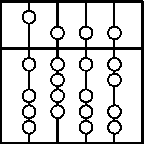
\includegraphics[width=2.4cm]{tum-abakus}

\end{center}

\newpage

%%%%%%%%%%%%%%%%%%%%%%%%%%%%%%%
% zweite Seite

\thispagestyle{empty}
\cleardoublepage 

%%%%%%%%%%%%%%%%%%%%%%%%%%%%%%%
% dritte Seite

\thispagestyle{empty}

\begin{center}


\includegraphics[width=3cm]{tum-logo}

\vspace{1cm}

{\Huge FAKULT�T F�R INFORMATIK\\[1mm]}
DER TECHNISCHEN UNIVERSIT�T M�NCHEN\\

\vspace{2cm}

{\Large \textbf{\typeOfThesis\ in Informatik}}\\

\vspace{2.0cm}
{\Huge \textbf{\titleOfThesisOne}}\\
\vspace*{3mm}
{\Huge \textbf{\titleOfThesisTwo}}\\
\vspace*{3mm}
{\Huge \textbf{\titleOfThesisThree}}\\

\vspace{1.5cm}

\parbox{1cm}{
  \begin{large}
    \begin{tabbing}
      Bearbeiter: \hspace{1cm}
        \=\authorOfThesis\\[2mm]
      Aufgabensteller:
        \>\aufgabensteller\\[2mm]
      Betreuer: 
        \>\betreuerOne\\
        \>\betreuerTwo\\
      Abgabedatum: 
        \> \abgabeTagZahl.~\abgabeMonatText~\abgabeJahrZahl\\
    \end{tabbing}
  \end{large}
}\\

\vspace{5mm}

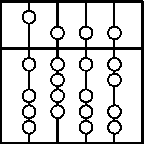
\includegraphics[width=2.4cm]{tum-abakus}

\end{center}
%
  \fi%
  \ifLMU%
    %
% LaTeX-Rahmen für Arbeiten am Lehrstuhl Hegering
%
% Harald Roelle, 2001, 2002
%
% basierend auf Arbeiten von Helmut Reiser, Boris Gruschke und Stephen Heilbronner
%


%Link im PDF
\ifpdf
  \pdfbookmark[0]{Titel}{Titel}%
\fi

%%%%%%%%%%%%%%%%%%%%%%%%%%%%%%%
% erste Seite

\thispagestyle{empty}

\begin{center}

\vspace*{-2cm}

{\Huge INSTITUT FÜR INFORMATIK\\[1mm]}
DER LUDWIG--MAXIMILIANS--UNIVERSITÄT MÜNCHEN\\

\vspace*{1cm}


\includegraphics[width=0.3\textwidth]{lmu_siegel}

\vspace*{2cm}

{\Large \textbf{\typeOfThesis}}\\

\vspace{2.0cm}
{\Huge \textbf{\titleOfThesisOne}}\\
\vspace*{3mm}
{\Huge \textbf{\titleOfThesisTwo}}\\
\vspace*{3mm}
{\Huge \textbf{\titleOfThesisThree}}\\

\vspace{1.5cm}

{\LARGE \authorOfThesis}\\[2mm]
{\LARGE \authorOfThesisOne}\\[2mm]
{\LARGE \authorOfThesisTwo}\\[2mm]

%\vspace{2cm}

%\parbox{1cm}{
%  \begin{large}
%    \begin{tabbing}
%      Aufgabensteller:
%        \=\aufgabensteller\\[2mm]
%      Betreuer: 
%        \>\betreuerOne\\
%        \>\betreuerTwo\\
%        \>\betreuerThree\\[5mm]
%      Abgabetermin: 
%        \> \abgabeTagZahl.~\abgabeMonatText~\abgabeJahrZahl\\
%    \end{tabbing}
%  \end{large}
%}\\

\end{center}

\newpage

%%%%%%%%%%%%%%%%%%%%%%%%%%%%%%%
% zweite Seite

\thispagestyle{empty}
\cleardoublepage 

%%%%%%%%%%%%%%%%%%%%%%%%%%%%%%%
% dritte Seite (Kopie der ersten)

\thispagestyle{empty}

\begin{center}

\vspace*{-2cm}

{\Huge INSTITUT FÜR INFORMATIK\\[1mm]}
DER LUDWIG--MAXIMILIANS--UNIVERSITÄT MÜNCHEN\\

\vspace*{1cm}


\includegraphics[width=0.3\textwidth]{lmu_siegel}

\vspace*{2cm}

{\Large \textbf{\typeOfThesis}}\\

\vspace{2.0cm}
{\Huge \textbf{\titleOfThesisOne}}\\
\vspace*{3mm}
{\Huge \textbf{\titleOfThesisTwo}}\\
\vspace*{3mm}
{\Huge \textbf{\titleOfThesisThree}}\\

\vspace{1.5cm}

{\LARGE \authorOfThesis}\\[2mm]
{\LARGE \authorOfThesisOne}\\[2mm]
{\LARGE \authorOfThesisTwo}\\[2mm]

\vspace{2cm}

\parbox{1cm}{
  \begin{large}
    \begin{tabbing}
      Aufgabensteller:
        \=\aufgabensteller\\[10mm]
      Abgabetermin: 
        \> \abgabeTagZahl.~\abgabeMonatText~\abgabeJahrZahl\\
    \end{tabbing}
  \end{large}
}\\

\end{center}
%
  \fi%
  
  % Erklärung
  %%
% LaTeX-Rahmen f�r Arbeiten am Lehrstuhl Hegering
%
% Harald Roelle, 2001, 2002
%
% basierend auf Arbeiten von Helmut Reiser, Boris Gruschke und Stephen Heilbronner
%

\newpage 

\thispagestyle{empty}

\begin{large}

\vspace*{2cm}
  
\noindent
Hiermit versichere ich, dass ich die vorliegende Diplomarbeit
selbst�ndig verfasst und keine anderen als die angegebenen Quellen
und Hilfsmittel verwendet habe.  

\vspace{2cm}

\noindent  
M�nchen, den \abgabeTagZahl.~\abgabeMonatText~\abgabeJahrZahl

\vspace{3cm}

\hspace*{7cm}%
\dotfill\\
\hspace*{8.5cm}%
\textit{(Unterschrift des Kandidaten)}

\end{large}
%
  
  % Abstract
  %\begin{DAabstract}%
  %  Hier steht eine kurze Zusammenfassung der Arbeit. Sie darf auf gar keinen Fall 
l�nger als eine Seite sein, ca. eine  halbe Seite ist optimal.

Das Abstract muss einfacher Plain-Text sein mit Leerzeile f�r Abs�tze. 
Grund: Daraus l�sst sich dann einfach der HTML-Text erzeugen, der automatisch
auf der Web-Page erscheint.
%
  %\end{DAabstract}%

  \pagestyle{empty}%
  \pagenumbering{roman}%
}

%
% Übergang von Verzeichnissen zum Hauptteil
%
\newcommand{\setupMainPart}[0]{%
  \cleardoublepage%
  \pagestyle{headings}%
  \pagenumbering{arabic}%
}

%
% Anhänge
%
\newcommand{\appendixbegin}[0]{%
  \cleardoublepage%
  \begin{appendix}%
  \setcounter{secnumdepth}{3}%
}
\newcommand{\appendixend}[0]{%
  \end{appendix}%
  \cleardoublepage%
}

%
% Wrapper fuer Literaturverzeichnis
%
\newcommand{\listofreferences}[0]{%
  \cleardoublepage%
  \bibliographystyle{geralpha-mnm-0.2} % Zitierungs-Richtlinien des Lehrstuhls
  \bibliography{\bibfiles}%
}

%
% Wrapper fuer Dokumentende
%
\newcommand{\docend}[0]{%
  \end{document}
}


%%% Local Variables: 
%%% mode: latex
%%% TeX-master: t
%%% End: 

\graphicspath{{Bilder/}}

%=============================================================================================
% Eigene Definitionen
%=============================================================================================

% Syntax-Definitionen für die Einbindung von Sourcecodes
\lstloadlanguages{C}
\lstloadlanguages{java}
\lstloadlanguages{make}

\lstset{language=sh, 
        keywordstyle=\ttfamily,
        commentstyle=\color{blue}, 
        breaklines=true,
        numbers=left, 
        numberstyle=\tiny, 
        stepnumber=2, 
        numbersep=5pt,
        captionpos=b,
        frame=single,
        linewidth=\linewidth,       % Zeilenbreite
	breaklines=true,             % Zeileumbruch
	literate=%
{Ö}{{\"O}}1
{Ä}{{\"A}}1
{Ü}{{\"U}}1
{ß}{{\ss}}2
{ü}{{\"u}}1
{ä}{{\"a}}1
{ö}{{\"o}}1
} 
	
%=============================================================================================
% Die Arbeit
%=============================================================================================

\docbegin            % MUSS STEHENBLEIBEN!


%
% Literatur, die nicht direkt im Text zitiert wird.
%
\nocite{han99}


%
% Diverse Verzeichnisse
%
%\setcounter{tocdepth}{2} % Begrenzen der Verzeichnistiefe
%\tableofcontents     % Inhaltsverzeichnis
%\listoffigures       % Liste aller Abbildungen
%\listoftables        % Liste aller Tabellen

\setupMainPart       % MUSS STEHENBLEIBEN!

%
% Kapitel
%
\chapter{Einleitung}

Primäre Zielsetzung unserer Versuche war es vorerst, \emph{virtualisierte
Maschinen} (VMs) auf der Praktikumsumgebung zu erstellen, und diese
zwischen Hostsystemen mittels Live-Migration zu verschieben. Dazu waren viele
Vorarbeiten und Versuche notwendig. Nachdem wir schließlich VMs erfolgreich migrieren konnten experimentierten wir mit
weiteren Möglichkeiten der Virtualisierung und verteilten Datenspeichern.

Die Ausarbeitung behandelt in den Kapiteln \ref{chap:whezzy_ugprade} bis \ref{chap:ovs} die Vorarbeiten
an der zur Virtualisierung genutzten Infrastruktur, die nötig sind um VMs zu erstellen.
Dies beginnt in Kapitel \ref{chap:whezzy_ugprade} mit einem Distributionsupgrade des Debiansystems, 
das zur Virtualisierung dienen soll, um neuere Versionen der genutzten Programme nutzen zu können. Anschließend wird in Kapitel \ref{chap:stor} ein Datenspeicher für die zukünftigen VMs geschaffen. Hierzu dient der \emph{Logical Volume Manager} (LVM) der auf einem darunter liegenden \emph{Redundant Array of Independent Disks} (RAID) aufgesetzt ist. Kapitel \ref{chap:ovs} beschäftigt sich mit der Erstellung eines Netzes für die Virtuellen Maschinen mittels \emph{Open vSwitch} (OVS).

Ab Kapitel \ref{vms} erstellten wir insgesamt vier VMs mit unterschiedlichen
Parametern und Einstellungen. Hierbei wurden, die Möglichkeit der rein in Software ablaufenden Paravirtualisierung und der Hardware-gestützten Vollvirtualisierung (Hardware Virtual Maschine -- HVM) betrachtet. Um später Live-Migrationen durchführen zu können ist es notwendig den Hintergrundspeicher der VMs über das Netz zur Verfügung zu stellen. Zu diesem Zweck wird in Kapitel \ref{chap:aoe} \emph{ATA-Over-Ethernet} (AoE) eingerichtet. Daraufhin finden in Kapitel \ref{migr} Versuche zur Live-Migration von VMs statt. Im Darauf folgenden Kapitel \ref{vlan_trunk} wird ein internes Netz, auf das nur die VMs zugriff haben, hostübergreifend mit Hilfe des OVS verfügbar gemacht. Den Abschluss der Arbeit bildet in Kapitel \ref{chap:drbd} ein Versuch ein \emph{Distributed Replicated Block Device} (DRBD) aufzubauen, bei dem mehrere Kopien eines Blockdevices hostübergreifend konsistent gehalten werden, um Ausfallsicherheit zu schaffen.

\chapter{Vorarbeit}
\label{chap:whezzy_ugprade}
Bevor mit dem eigentlichen Praktikum begonnen wurde, haben wir einige Vorarbeiten erledigt: \\ 
Um aktuellere Versionen von Xen einsetzen zu können, haben wir mit einem Distributionsupgrade des Praktikumssystems von Debian Squeeze auf Wheezy begonnen. \\ 
Dazu wird in \verb#/etc/apt/sources.list# jedes Vorkommen von \textquotedblleft\verb#squeeze#\textquotedblright ~ durch \textquotedblleft\verb#wheezy#\textquotedblright ~ ersetzt und folgende Befehle ausgeführt: 

\setupVerbatim{bash}
\begin{verbatim}
apt-get update
apt-get dist-upgrade -y
\end{verbatim}
Zusätzlich haben wir einen Symlink 
\setupVerbatimOut 
\begin{verbatim} 
09_linux_xen -> 20_linux_xen 
\end{verbatim} 
in \verb#/etc/grub.d# erstellt, damit der Xen Hypervisor standardmäßig geladen wird.
\\
Um die Konnektivität zum internen Netz der VMs nach dem Bootvorgang zu gewährleisten, haben wir die Konfiguration in \verb#/etc/network/interfaces# um \verb#eth0# erweitert. Darüber hinaus wurde der Nameserver in \verb#/etc/resolv.conf# auskommentiert, da dieser Probleme beim Auflösen von DNS-Einträgen außerhalb der Praktikumsumgebung hatte.

Der nächste Schritt ist nun die Einrichtung eines Datenspeichers für unsere Virtuellen Maschinen.

\chapter{Storage}\label{chap:stor}
Um einen Datenspeicher für spätere virtuelle Maschinen zu erhalten, entschlossen wir uns einen \emph{Redundant Array of Independent Disks} (RAID) Verbund über zwei Festplatten zu erzeugen (vgl. Abschnitt \ref{raid}). Wir entschieden uns für RAID Level 1. Dieser bietet durch die Spiegelung der Partitionen eine gewisse Daten- und Ausfallsicherheit. Als tatsächlicher Datenspeicher sollten schließlich mit dem \emph{Logical Volume Manager} (LVM) erzeugte \emph{Logical Volumes} (LV) dienen, was in Abschnitt \ref{lvm} umgesetzt wird.
\section{RAID}
\label{raid}
Für einen RAID-Verbund werden mindestens zwei Festplatten benötigt, welche möglichst identisch sein sollten. Wir verwenden die Platten \verb#sdb# und \verb#sdc# auf \verb#pcvirt01#. \\
Zum Erzeugen einer \emph{GUID Partition Table} (GPT) nutzten wir \verb#gdisk#, welches vorher installiert werden musste. \\ 
Zur reinen Erzeugung eines RAID Systems ist dies nicht zwingend erforderlich, jedoch stellt GPT den designierten Nachfolgestandard für MBR-Partitionstabellen dar. Ein paar der Vorteile einer GPT Partitionstabelle gegenüber einer MBR Partitionstabelle sind\cite{gpt}:
\begin{itemize} 
\item die Unterstützung von Laufwerken mit bis zu $2^{64}$ Sektoren,
\item die Redundanz der Tabelle am Ende der Festplatte, die vor dem Verlust der Tabelle im Falle eines defekten Sektors schützt,
\item die Absicherung der kritischen Bereiche der Tabelle mittels CRC
\end{itemize}
\setupVerbatim{bash}
\begin{verbatim}
apt-get install gdisk
gdisk /dev/sdb
\end{verbatim}
Auf \verb#/dev/sdb# wurden daraufhin zwei Partitionen erzeugt. Die erste für GPT mit ca. 1 Megabyte. Die zweite mit dem restlichen Platz der Festplatte.
Diese Partitionstabelle wurde mit \verb#sgdisk -R# auf die 2. Platte übertragen und danach dessen GUID mit \verb#sgdisk -G# wieder randomisiert.
\setupVerbatim{bash}
\begin{verbatim}
sgdisk -R=/dev/sdc /dev/sdb
sgdisk -G /dev/sdb
\end{verbatim}
Abschließend wurde der RAID-Verbund \verb#/dev/md1# über die beiden Partitionen \verb#/dev/sdb2# und \verb#/dev/sdc2# mit \verb#mdadm# erzeugt. Der Parameter \verb#-n# bezeichnet die Anzahl der Partitionen und \verb#-l# gibt den RAID Level an.
\setupVerbatim{bash}
\begin{verbatim}
mdadm --create /dev/md1 -n 2 -l 1 /dev/sdb2 /dev/sdc2
\end{verbatim}
Die Erstellung des RAID-Verbundes ist anhand der Ausgabe von \verb#dmesg# nachvollziehbar. Zur Überprüfung, ob die Erstellung erfolgreich war, ist der Inhalt von \verb#/proc/mdstat# hilfreich: 
\setupVerbatimOut
\begin{verbatim}
$ dmesg | tail
[  253.106706] sdb: sdb1 sdb2
[  364.210743] sdc: sdc1 sdc2
[  373.659167] sdb: sdb1 sdb2
[  701.414204] md: bind<sdb2>
[  701.415194] md: bind<sdc2>
[  701.425611] md: raid1 personality registered for level 1
[  701.425853] bio: create slab <bio-1> at 1
[  701.425897] md/raid1:md1: not clean -- starting background reconstruction
[  701.425898] md/raid1:md1: active with 2 out of 2 mirrors
[  701.425913] md1: detected capacity change from 0 to 499971325952
[  701.433300] md1: unknown partition table
[ 1223.952091] md: resync of RAID array md1
[ 1223.952093] md: minimum _guaranteed_  speed: 1000 KB/sec/disk.
[ 1223.952095] md: using maximum available idle IO bandwidth (but not more than 200000 KB/sec) for resync.
[ 1223.952097] md: using 128k window, over a total of 488253248k.

$ cat /proc/mdstat
Personalities : [raid1] 
md1 : active raid1 sdc2[1] sdb2[0]
      488253248 blocks super 1.2 [2/2] [UU]
      
unused devices: <none>
\end{verbatim}

Aus der Zeile \verb#md1 : active raid1 sdc2[1] sdb2[0]# lässt sich ablesen, dass das RAID-Device verfügbar ist. \verb#[UU]# zeigt an, dass beide gespiegelte Partitionen aktuell (Up) sind \cite{wiki_mdstat}.

\section{LVM}
\label{lvm}
Aufbauend auf dem RAID-Device haben wir ein LVM-System angelegt. Dazu wurde der soeben generierte RAID1-Verbund \verb#/dev/md1# aus Abschnitt \ref{raid} mit \verb#pvcreate# als Physical Volume (PV) initialisiert und mit \verb#vgcreate# in eine neue Volume Group \verb#storage# eingebunden. 
Dann haben wir mit \verb#lvcreate# zwei LVs in dieser Gruppe erstellt. Dabei gibt der Parameter \verb#-n# den Namen des LVs an, \verb#-L# die Größe. 
\setupVerbatim{bash}
\begin{verbatim}
pvcreate /dev/md1 
vgcreate storage /dev/md1
lvcreate -n guest1 -L 10G storage
lvcreate -n guest2 -L 20G storage
\end{verbatim} 
Mit dem Befehl \verb#lvm# kann der Status der Konfiguration überprüft werden. Dabei zeigt der Kommando \verb#lvs# Informationen der Logical Volumes und \verb#pvs# Informationen der Physical Volumes an. 
\setupVerbatimOut
\setupVerbatim{bash}
\begin{verbatim}
lvm> lvs
  LV               VG      Attr     LSize   Pool Origin Data%  Move Log Copy%  Convert                                        
  guest1           storage -wi-ao--  10.00g                                           
  guest2           storage -wi-ao--  20.00g                                           
lvm> pvs
  PV         VG      Fmt  Attr PSize   PFree  
  /dev/md1   storage lvm2 a--  465.63g 436.13g
\end{verbatim} 
Beim Erstellen der VMs haben wir festgestellt, dass dabei neue Partitionen für die Gastbetriebssysteme angelegt werden (\verb#guestX-disk# und \verb#guestX-swap#). Somit ist es also nicht notwendig diese von Hand zu erstellen. 

\chapter{Open vSwitch}
\label{chap:ovs}
Da wir die von Linux mitgelieferte Bridge-Implementierung durch Open vSwitch (OVS) ersetzen wollten, waren einige weitere Schritte notwendig. Die Vorteile, die Open vSwitch im Bereich VLAN-Trunking bringt, welches in Kapitel \ref{vlan_trunk} eingesetzt werden soll, wiegen diese Zusatzarbeiten unserer damaligen Einschätzung nach auf.
\\
Die Installation gestaltet sich auf dem Debian Wheezy System relativ einfach, da mit \verb#apt-get# die Pakete problemlos geladen werden können:
\setupVerbatim{bash}
\begin{verbatim}
apt-get install openvswitch-brcompat openvswitch-switch openvswitch-datapath-dkms
\end{verbatim}

Ein anschließendes \verb#modprobe openvswitch-mod# lädt das Kernelmodul von Open vSwitch. Dessen erfolgreiche Installation kann man der Ausgabe von \verb#dmesg# entnehmen:
\setupVerbatimOut
\begin{verbatim}
[ 2377.104677] openvswitch_mod: Open vSwitch switching datapath 1.4.2, built Apr 30 2013 15:47:50
\end{verbatim}
Das Paket \verb#openvswitch-brcompat# bietet eine Unterstützung für Programme, die bislang das Kommando \verb#brctl# des \verb#bridge# Moduls nutzten, um mit Open vSwitch weiterhin zu funktionieren. Damit diese Unterstützung aktiviert wird, musste in der Datei \verb#/etc/default/openvswitch-switch# der Schalter \verb#BRCOMPAT=yes# gesetzt werden. Anschließend wurde der OVS-Dienst gestartet und eine Bridge für die VMs erzeugt:
\setupVerbatimBash
\begin{verbatim}
/etc/init.d/openvswitch-switch start
ovs-vsctl add-br br-guest
\end{verbatim}
Die erfolgreiche Erstellung kann mittels \verb#ovs-vsctl show# überprüft werden:
\setupVerbatimOut
\begin{verbatim}
b01c6804-1ad5-4294-98d1-b6aa0a8f6155
    Bridge br-guest
        Port br-guest
            Interface br-guest
                type: internal
    ovs_version: "1.4.2"
\end{verbatim} 
Um eine Verbindung der Bridge in die physische Welt zu schaffen, musste eine physische Schnittstelle zur Bridge hinzugefügt werden.
\setupVerbatimBash
\begin{verbatim}
ovs-vsctl add-port br-guest eth0
\end{verbatim}
Das Ergebnis wurde abermals mit \verb#ovs-vsctl show# überprüft:
\setupVerbatimOut
\begin{verbatim}
b01c6804-1ad5-4294-98d1-b6aa0a8f6155
     Bridge br-guest
        Port "eth0"
            Interface "eth0"
        Port br-guest
            Interface br-guest
                type: internal
    ovs_version: "1.4.2"
\end{verbatim}

Anschließend wurde die Konfiguration der Schnittstellen in \verb#/etc/network/interfaces# angepasst, damit anstatt dem einzelnen Interface \verb#eth0# beim Start des Systems die Bridge \verb#br-guest# konfiguriert wird:
\setupVerbatimOut
\begin{verbatim}
auto lo eth1

# The loopback network interface
iface lo inet loopback

# The primary network interface
iface eth1 inet static
    address 10.163.235.131
    netmask 255.255.255.128
    gateway 10.163.235.254

auto br-guest
iface br-guest inet static
    address 192.168.1.131
    netmask 255.255.255.0
    bridge_ports eth0
\end{verbatim}

Die oben getätigten Einstellungen des \verb#ovs-vsctl# Kommandos werden ohne weiteres Zutun durch Open vSwitch persistent gespeichert. Dies stellt einen Vorteil im Vergleich zur klassischen Linux Bridge dar. Dies alleine rechtfertigt schon den Aufwand zur Installation von Open vSwitch. 
\\
Anschließend wurde die Konfiguration, durch einen Neustart geladen. Die Konnektivität zu anderen Hosts im internen Praktikumsnetz wurde mittels \verb#ping# erfolgreich überprüft.
\\
\\
Die grundlegenden Anforderungen an die Infrastruktur des Hostrechners sind damit erfüllt, sodass im nächsten Kapitel die erste VM erstellt werden kann.

\chapter{Virtuelle Maschinen}\label{vms}
Nachdem nun alle notwendigen Vorbereitungen abgeschlossen waren, konnte die erste \emph{virtuelle Maschine} (VM) erstellt werden. Dazu wurde das Kommando \verb#xen-create-image# genutzt, welches die Erstellung einer paravirtualisierten VM weitestgehend automatisiert. Es wird zuerst die VM \verb#guest1# mit dem Betriebssystem Debian Wheezy, anschließend dann \verb#guest2# mit Debian Squeezy erstellt.
\\
Im Abschnitt \ref{hvm_vm} wird dann eine vollvirtualisierte VM \verb#guest4# wiederum mit Debian Wheezy erstellt. Bei dieser Vollvirtualisierung läuft das Gastbetriebssystem prinzipiell ohne Anpassungen an den Hypervisor. Um IO-Operationen zu beschleunigen werden jedoch spezielle Treiber für Netzschnittstellen und Festplatten verwendet. 
\\
Die Performanz der verschiedenen Virtualisierungsmethoden bei Netzschnittstellen wird im letzten Abschnitt des Kapitels (Abschnitt \ref{perf}) anhand eines Experimentes untersucht.

\section{Erstellung einer paravirtualisierten VM}
Um die ersten paravirtualisierten VMs auf dem Host \verb#pcvirt01# zu erzeugen, wurde das Skript \verb#xen-create-image# genutzt. Diesem kann man über diverse Parameter Einstellungen übergeben. Des weiteren übernimmt es die Installation der paravirtualisierten Gastbetriebssysteme für den Nutzer.
\setupVerbatim{bash}
\begin{verbatim}
xen-create-image --ip 192.168.10.12  --lvm=storage --hostname=guest1 --vcpus=2 --dist wheezy
\end{verbatim}
\setupVerbatimOut
\begin{verbatim}                                                  
WARNING                                           
-------                                           
                                                  
  You appear to have a missing vif-script, or network-script, in the
 Xen configuration file /etc/xen/xend-config.sxp. 
                                                  
  Please fix this and restart Xend, or your guests will not be able
 to use any networking!                           
                                                  
WARNING:  No gateway address specified!           
WARNING:  No netmask address specified!           
                                                  
General Information                               
--------------------                              
Hostname       :  guest1                          
Distribution   :  wheezy                          
Mirror         :  http://cdn.debian.net/debian/   
Partitions     :  swap            128Mb (swap)    
                  /               4Gb   (ext3)    
Image type     :  full                            
Memory size    :  128Mb                           
Kernel path    :  /boot/vmlinuz-3.2.0-4-amd64     
Initrd path    :  /boot/initrd.img-3.2.0-4-amd64  
                                                  
Networking Information                            
----------------------                            
IP Address 1   : 192.168.10.12 [MAC: 00:16:3E:95:61:15]
                                                  
                                                  
Creating swap on /dev/storage/guest1-swap         
Done                                              
                                                  
Creating ext3 filesystem on /dev/storage/guest1-disk
Done                                              
Installation method: debootstrap
Done

Running hooks
Done

No role scripts were specified.  Skipping

Creating Xen configuration file
Done

No role scripts were specified.  Skipping
Setting up root password
Generating a password for the new guest.
All done


Logfile produced at:
         /var/log/xen-tools/guest1.log

Installation Summary
---------------------
Hostname        :  guest1
Distribution    :  wheezy
IP-Address(es)  :  192.168.10.12 
RSA Fingerprint :  01:06:31:35:f0:d4:f0:70:54:d3:0f:f2:d4:90:ba:e1
Root Password   :  JzXi4Ufg
\end{verbatim}

Anschließend haben wir die Konfiguration \verb#/etc/xen/guest1.cfg# der VM noch von Hand angepasst um die Anzahl der CPUs zu verändern und mehr Arbeitsspeicher zu erhalten:
\setupVerbatimOut
\begin{verbatim}
    vcpus       = '3'
    memory      = '512'
\end{verbatim}

Abschließend wurde die VM gestartet:
\setupVerbatim{bash}
\begin{verbatim}
xm create /etc/xen/guest1.cfg
\end{verbatim}

Auf dem Host wurde hierdurch eine Schnittstelle \verb#vif1.0# erstellt und mit der Bridge \verb#br-guest# verbunden. Nach dem Wechsel in die Konsole der VM mittels \verb#xm# \verb#console# \verb#guest1# wurde die Konnektivität zum Host mittels \verb#ping# auf der VM erfolgreich überprüft. Zum Verlassen der Konsole dient \verb#Ctrl+AltGr+9#.

\section{Weitere VM und Bridge für VM-Interconnect}
Der nächste Versuch erweiterte den aktuellen Aufbau um eine weitere VM und eine zusätzliche Bridge. Diese verbindet ausschließlich Schnittstellen der VMs und besitzt keine Anbindung an ein physisches Interface. Später soll diese Bridge über ein VLAN auch VMs auf zwei verschiedenen Hosts verbinden.
\setupVerbatim{bash}
\begin{verbatim}
xen-create-image --ip 192.168.10.13  --lvm=storage --hostname=guest2 --vcpus=2 --bridge=br-guest
ovs-vsctl add-br br-vmonly
\end{verbatim}
Um ein weiteres Interface auf der Bridge br-vmonly zu erhalten wurde die soeben erstellte Konfiguration \verb#/etc/xen/guest2.cfg# angepasst:
\setupVerbatimOut
\begin{verbatim}
vif         = [
    'mac=00:16:3E:32:D0:3E,bridge=br-guest',
    'mac=00:16:3E:32:CA:FE,bridge=br-vmonly' 
             ]
\end{verbatim}
Auf \verb#guest1# geschah das Hinzufügen des 2. Interfaces analog.\\
Anschließend wurden die VMs gestartet und die Datentransferrate zwischen den VMs mittels \verb#iperf# bestimmt. Die gemessenen Übertragungsraten in der Größenordnung von 8 $\frac{Gbit}{s}$ und sind damit deutlich höher als bei Vergleichsmessungen zwischen einer VM und einem anderen physischen System.

\setupVerbatimOut
\begin{verbatim}
------------------------------------------------------------
Client connecting to 192.168.2.2, TCP port 5001
TCP window size: 23.5 KByte (default)
------------------------------------------------------------
[  3] local 192.168.2.1 port 57804 connected with 192.168.2.2 port 5001
[ ID] Interval       Transfer     Bandwidth
[  3]  0.0-10.0 sec  9.21 GBytes  @\bfseries 7.91@ @\bfseries Gbits/sec@


------------------------------------------------------------
Client connecting to 192.168.1.2, TCP port 5001
TCP window size: 23.5 KByte (default)
------------------------------------------------------------
[  3] local 192.168.1.1 port 56132 connected with 192.168.1.2 port 5001
[ ID] Interval       Transfer     Bandwidth
[  3]  0.0-10.0 sec  10.6 GBytes  @\bfseries 9.12@ @\bfseries Gbits/sec@
\end{verbatim}
Ein nebenbei laufender \verb#tcpdump# auf dem empfangenden System zeigte sehr große eingehende Ethernet-Frames mit Größen bis zu 65226 Byte: 
\setupVerbatimOut
\begin{verbatim}
17:45:48.414535 00:16:3e:32:d0:3e > 00:16:3e:95:de:ad, ethertype IPv4 (0x0800), @\bfseries length@ @\bfseries 65226@: (tos 0x0, ttl 64, id 25535, offset 0, flags [DF], proto TCP (6), @\bfseries length@ @\bfseries 65212@)
    192.168.1.2.57025 > 192.168.1.1.5001: Flags [.], seq 14811337:14876497, ack 0, win 913, options [nop,nop,TS val 396548 ecr 356977], @\bfseries length@ @\bfseries 65160@
17:45:48.414540 00:16:3e:32:d0:3e > 00:16:3e:95:de:ad, ethertype IPv4 (0x0800), @\bfseries length@ @\bfseries 65226@: (tos 0x0, ttl 64, id 25580, offset 0, flags [DF], proto TCP (6), @\bfseries length@ @\bfseries 65212@)
    192.168.1.2.57025 > 192.168.1.1.5001: Flags [P.], seq 14876497:14941657, ack 0, win 913, options [nop,nop,TS val 396548 ecr 356977], @\bfseries length@ @\bfseries 65160@
17:45:48.414542 00:16:3e:32:d0:3e > 00:16:3e:95:de:ad, ethertype IPv4 (0x0800), @\bfseries length@ @\bfseries 65226@: (tos 0x0, ttl 64, id 25625, offset 0, flags [DF], proto TCP (6), @\bfseries length@ @\bfseries 65212@)
    192.168.1.2.57025 > 192.168.1.1.5001: Flags [.], seq 14941657:15006817, ack 0, win 913, options [nop,nop,TS val 396548 ecr 356977], @\bfseries length@ @\bfseries 65160@
17:45:48.414559 00:16:3e:95:de:ad > 00:16:3e:32:d0:3e, ethertype IPv4 (0x0800), length 66: (tos 0x0, ttl 64, id 54265, offset 0, flags [DF], proto TCP (6), length 52)
    192.168.1.1.5001 > 192.168.1.2.57025: Flags [.], cksum 0x837a (@\bfseries incorrect@ -> 0x86f4), seq 0, ack 14876497, win 16397, options [nop,nop,TS val 356977 ecr 396548], length 0
\end{verbatim}
Wohingegen Ping-Pakete, welche die MTU der \verb#vif#-Schnittstellen oder Bridges überschritten fragmentiert -- oder bei gesetztem \verb#DF#-Flag abgewiesen -- wurden.
Dies liegt daran, dass die Treiber der virtualisierten Schnittstellen dem Kernel mitteilen sie würden \emph{TCP Segment Offloading} (TSO) unterstützen. Bei dieser Technik übernimmt die Schnittstelle die Segmentierung der TCP-Daten. Im Fall der Virtualisierung werden die unsegmentierten TCP-Daten an den Hypervisor übergeben und in diesem entweder vor der Übertragung auf physische Schnittstellen segmentiert oder wiederum unsegmentiert an andere auf diesem Host laufende Gastbetriebssysteme weitergegeben. Die \verb#cksum# \verb#incorrect# Meldung entsteht ebenso durch eine Offloadingtechnik. Hierbei werden die Ethernet-Checksummen von der Schnittstelle und nicht dem OS gesetzt. 
Zusätzlich wurde getestet, ob die Bridges und \verb#vif#-Schnittstellen mit Jumbo-Frames von 9000 Byte Größe umgehen können. Nach Erhöhung der MTU auf der Bridge, den \verb#vif#-Schnittstellen und auf den Schnittstellen des Gastes konnten Jumbo-Frames genutzt werden.

\section{Hardware Virtual Machine}
\label{hvm_vm}
Neben der Paravirtualisierung unterstützt Xen auch noch Vollvirtualiserung. Hierzu wird von Xen mit Hilfe der Virtualisierungsunterstützung der CPU ein Hypervisor installiert, der die Traps abfängt und die entsprechenden Hypercalls am eigentlichen Xen-Hypervisor aufruft.

Um eine vollvirtualisierte VM zu erstellen, muss die Konfiguration der VM angepasst werden (gekürzte Darstellung):
\setupVerbatimOut
\begin{verbatim}
kernel      = '/usr/lib/xen-4.1/boot/hvmloader'
builder     = 'hvm'
device_model= '/usr/lib/xen-4.1/bin/qemu-dm'

vnc=1
vncconsole=1
vnclisten='0.0.0.0'
vncpasswd=''
keymap='de'
\end{verbatim}

Durch die Konfiguration des Kernels zu \verb#hvmloader# und Nutzung des Builders \verb#hvm# wird eine Vollvirtualisierung angestoßen. Die VNC-Konfiguration ist notwendig, um die grafische Ausgabe der VM sehen zu können. Eine Betriebssysteminstallation kann beispielsweise durch Hinzufügen eines ISO-Images als CDROM-Laufwerk ermöglicht werden: 
\setupVerbatimOut
\begin{verbatim}
disk = [ <WEITERE KONFIGURATION> , 'file:/xen/iso/debian-7.0.0-amd64-netinst.iso,hdc:cdrom,r']
\end{verbatim}

\section{Netzperformanz unterschiedlicher VM Typen}\label{perf}

Nun wird durch ein Experiment die Netzperformanz verschiedener VM-Typen mittels \verb#iperf# zwischen Hostmaschine und VM gemessen. Es wird zwischen folgenden Schnittstellentypen unterschieden:
\begin{itemize}
\item paravirtualisierte VM (PVM)
\item vollvirtualisierte VM mit Netzschnittstellenemulation durch \verb#QEMU# (HVM)
\item vollvirtualisierte VM mit paravirtualisierten Netzschnittstellen-Treibern (HVM\_PV)
\end{itemize}

Dieser Test zeigt wie in Abbildung \ref{megaplot} ersichtlich signifikante Unterschiede bzgl. der Datenraten. Während die Messung mit HVM\_PV-Treibern -- die standardmäßig aktiviert sind -- ebenso wie die PVM hohe Datenraten zeigen, bricht die Datenrate bei der \verb#QEMU#-Emulation erheblich ein.
\\
Den Verzicht auf die HVM\_PV-Treiber konfiguriert man mit dem Parameter \verb#xen_platform_pci = 0# in der Konfigurationsdatei der VM.

Die jetzige Konfiguration des Hostsystems \verb#pcvirt01# kann somit VMs erfolgreich ausführen. Damit man nun VMs auf ein weiteres Hostsystem übertragen kann, muss auch von diesem der Hintergrundspeicher der jeweiligen VM erreichbar sein. Da dieser derzeit nur von \verb#pcvirt01# aus erreichbar ist, muss man in einem weiteren Schritt diesen über das Praktikumsnetz freigeben.
\begin{figure}
\begin{tikzpicture}[trim axis left]
    \begin{axis}[
    	change y base,
    	y SI prefix=giga,
        width=0.9\textwidth,
        x unit=s,
        xlabel=Zeit,
        y unit=Bit/s,
        ylabel=Datenrate,
        legend pos=outer north east]
    \addplot[smooth,mark=*,blue] plot coordinates {
    (0.000000,13055800832)
    (0.500000,12688813056)
    (1.000000,12330210304)
    (1.500000,12352225280)
    (2.000000,13154379904)
    (2.500000,12437178880)
    (3.000000,13284390400)
    (3.500000,13259249536)
    (4.000000,13236168832)
    (4.500000,13248775808)
    (5.000000,13248740608)
    (5.500000,13226749696)
    (6.000000,13050564864)
    (6.500000,13019118720)
    (7.000000,13238278016)
    (7.500000,12856597248)
    (8.000000,13223585024)
    (8.500000,13230944000)
    (9.000000,13230919936)
    (9.500000,13202614400)
    (10.000000,13291749376)
    (10.500000,13256097792)
    (11.000000,13219403648)
    (11.500000,13286501376)
    (12.000000,13211014144)
    (12.500000,13312720896)
    (13.000000,13211003904)
    (13.500000,13216251008)
    (14.000000,13117685760)
    (14.500000,12847153152)
    (15.000000,13203668992)
    (15.500000,13262390144)
    (16.000000,13301191680)
    (16.500000,13266584448)
    (17.000000,13315859712)
    (17.500000,13113491456)
    (18.000000,13214154752)
    (18.500000,12616467328)
    (19.000000,13231986560)
    (19.500000,13238265984)
    (20.000000,13216251008)
    (20.500000,13295943680)
    (21.000000,13239321472)
    (21.500000,13188988032)
    (22.000000,13265540992)
    (22.500000,13282307072)
    (23.000000,13230931072)
    (23.500000,12846110592)
    (24.000000,13222544256)
    (24.500000,13202626432)
    (25.000000,13231973632)
    (25.500000,13243526912)
    (26.000000,13262378112)
    (26.500000,13165920256)
    (27.000000,12870220928)
    (27.500000,13012829056)
    (28.000000,13223585920)
    (28.500000,13324272384)
    (29.000000,13034843136)
    (29.500000,13271819520)
    };
    \addlegendentry{PVM $\rightarrow$ Host}

    \addplot[smooth,color=blue,mark=x]
        plot coordinates {
   		(0.000000,5047844864)
    (0.500000,5337251840)
    (1.000000,6155141120)
    (1.500000,6167724032)
    (2.000000,5052039168)
    (2.500000,5884608512)
    (3.000000,4995416064)
    (3.500000,4976541696)
    (4.000000,4963958784)
    (4.500000,4970250240)
    (5.000000,4984930304)
    (5.500000,4959764480)
    (6.000000,5119148032)
    (6.500000,5196742656)
    (7.000000,5047844864)
    (7.500000,5018484736)
    (8.000000,4945084416)
    (8.500000,4963958784)
    (9.000000,4945084416)
    (9.500000,4945084416)
    (10.000000,4972347392)
    (10.500000,4953473024)
    (11.000000,4936695808)
    (11.500000,4972347392)
    (12.000000,4945084416)
    (12.500000,4991221760)
    (13.000000,4936695808)
    (13.500000,4953473024)
    (14.000000,5060427776)
    (14.500000,5427429376)
    (15.000000,4934598656)
    (15.500000,4963958784)
    (16.000000,4982833152)
    (16.500000,4963958784)
    (17.000000,4972347392)
    (17.500000,4915724288)
    (18.000000,4936695808)
    (18.500000,5676990464)
    (19.000000,4945084416)
    (19.500000,4955570176)
    (20.000000,4963958784)
    (20.500000,4982833152)
    (21.000000,4953473024)
    (21.500000,4934598656)
    (22.000000,4974444544)
    (22.500000,4972347392)
    (23.000000,4966055936)
    (23.500000,5261754368)
    (24.000000,4955570176)
    (24.500000,4945084416)
    (25.000000,4963958784)
    (25.500000,4978638848)
    (26.000000,4972347392)
    (26.500000,5056233472)
    (27.000000,5429526528)
    (27.500000,4888461312)
    (28.000000,4945084416)
    (28.500000,5010096128)
    (29.000000,5247074304)
        };
    \addlegendentry{Host $\rightarrow$ PVM}
    
    \addplot[smooth,mark=*,red] plot coordinates {
(0.000000,9964599680)
    (0.500000,10250878080)
    (1.000000,10237254400)
    (1.500000,10241434880)
    (2.000000,10276045696)
    (2.500000,10257169536)
    (3.000000,10271850496)
    (3.500000,10298070912)
    (4.000000,10278153984)
    (4.500000,10285463936)
    (5.000000,10306447488)
    (5.500000,10237254400)
    (6.000000,10234112896)
    (6.500000,10295961728)
    (7.000000,10330570752)
    (7.500000,10302253184)
    (8.000000,10285488000)
    (8.500000,10249824384)
    (9.000000,10249825280)
    (9.500000,10271849600)
    (10.000000,10214184832)
    (10.500000,10313793536)
    (11.000000,10207893376)
    (11.500000,10168036352)
    (12.000000,10257181568)
    (12.500000,10286519424)
    (13.000000,10245641216)
    (13.500000,10267656192)
    (14.000000,10252988160)
    (14.500000,10252964096)
    (15.000000,10300156928)
    (15.500000,10290724864)
    (16.000000,10306458624)
    (16.500000,10270796800)
    (17.000000,10295972864)
    (17.500000,10316934144)
    (18.000000,10325333888)
    (18.500000,10245629184)
    (19.000000,10242502400)
    (19.500000,10246684672)
    (20.000000,9234802816)
    (20.500000,10286519424)
    (21.000000,10282348288)
    (21.500000,10301210624)
    (22.000000,10279183616)
    (22.500000,10270807936)
    (23.000000,10249824384)
    (23.500000,9772729216)
    (24.000000,10268709888)
    (24.500000,10286531456)
    (25.000000,10265571072)
    (25.500000,10233047168)
    (26.000000,10268686720)
    (26.500000,10283390848)
    (27.000000,10186920960)
    (27.500000,10293865472)
    (28.000000,10221517952)
    (28.500000,10259267584)
    (29.000000,10201601920)
    (29.500000,10278154880)
    };
    \addlegendentry{HVM\_PV $\rightarrow$ Host}

    \addplot[smooth,color=red,mark=x] plot coordinates {
(0.000000,4435476480)
    (0.500000,4341104640)
    (1.000000,4301258752)
    (1.500000,4324327424)
    (2.000000,4286578688)
    (2.500000,4294967296)
    (3.000000,4292870144)
    (3.500000,4271898624)
    (4.000000,4292870144)
    (4.500000,4282384384)
    (5.000000,4280287232)
    (5.500000,4341104640)
    (6.000000,4318035968)
    (6.500000,4297064448)
    (7.000000,4280287232)
    (7.500000,4280287232)
    (8.000000,4273995776)
    (8.500000,4309647360)
    (9.000000,4320133120)
    (9.500000,4301258752)
    (10.000000,4303355904)
    (10.500000,4263510016)
    (11.000000,4347396096)
    (11.500000,4315938816)
    (12.000000,4305453056)
    (12.500000,4292870144)
    (13.000000,4278190080)
    (13.500000,4320133120)
    (14.000000,4324327424)
    (14.500000,4297064448)
    (15.000000,4250927104)
    (15.500000,4294967296)
    (16.000000,4280287232)
    (16.500000,4309647360)
    (17.000000,4276092928)
    (17.500000,4271898624)
    (18.000000,4261412864)
    (18.500000,4324327424)
    (19.000000,4313841664)
    (19.500000,4330618880)
    (20.000000,4462739456)
    (20.500000,4307550208)
    (21.000000,4297064448)
    (21.500000,4299161600)
    (22.000000,4339007488)
    (22.500000,4330618880)
    (23.000000,4309647360)
    (23.500000,4418699264)
    (24.000000,4299161600)
    (24.500000,4255121408)
    (25.000000,4278190080)
    (25.500000,4343201792)
    (26.000000,4282384384)
    (26.500000,4282384384)
    (27.000000,4334813184)
    (27.500000,4269801472)
    (28.000000,4345298944)
    (28.500000,4322230272)
    (29.000000,4397727744)
    (29.500000,4387241984)
        };
    \addlegendentry{Host $\rightarrow$ HVM\_PV}
    
    \addplot[smooth,mark=*,green] plot coordinates {
	(0.000000,456135680)
    (0.500000,448500480)
    (1.000000,450737536)
    (1.500000,442649216)
    (2.000000,445871360)
    (2.500000,432603648)
    (3.000000,438305664)
    (3.500000,420714880)
    (4.000000,329832960)
    (4.500000,420832512)
    (5.000000,397787008)
    (5.500000,394276608)
    (6.000000,366642048)
    (6.500000,369295232)
    (7.000000,383929856)
    (7.500000,337270784)
    (8.000000,380708608)
    (8.500000,450701440)
    (9.000000,420902016)
    (9.500000,458292096)
    (10.000000,451895936)
    (10.500000,443575936)
    (11.000000,452232320)
    (11.500000,411481088)
    (12.000000,454202496)
    (12.500000,455231232)
    (13.000000,453738240)
    (13.500000,455627776)
    (14.000000,454235008)
    (14.500000,443113472)
    (15.000000,454756736)
    (15.500000,297401728)
    (16.000000,447922176)
    (16.500000,446159616)
    (17.000000,451677184)
    (17.500000,364115840)
    (18.000000,445650816)
    (18.500000,445894528)
    (19.000000,425466112)
    (19.500000,449172352)
    (20.000000,452614144)
    (20.500000,445442304)
    (21.000000,360907520)
    (21.500000,398457984)
    (22.000000,388101888)
    (22.500000,387844352)
    (23.000000,444145792)
    (23.500000,383221888)
    (24.000000,382689920)
    (24.500000,382330368)
    (25.000000,365310336)
    (25.500000,428514048)
    (26.000000,449206656)
    (26.500000,453958784)
    (27.000000,423647872)
    (27.500000,443541632)
    (28.000000,454804864)
    (28.500000,453969024)
    (29.000000,451803264)
    (29.500000,458105856)
    };
    \addlegendentry{HVM $\rightarrow$ Host}
\addplot[smooth,color=green,mark=x] plot coordinates {
(0.000000,8388608)
    (0.500000,8388608)
    (1.000000,12582912)
    (1.500000,14680064)
    (2.000000,4194304)
    (2.500000,6291456)
    (3.000000,4194304)
    (3.500000,4194304)
    (4.000000,48234496)
    (4.500000,58720256)
    (5.000000,81788928)
    (5.500000,83886080)
    (6.000000,100663296)
    (6.500000,104857600)
    (7.000000,111149056)
    (7.500000,98566144)
    (8.000000,125829120)
    (8.500000,4194304)
    (9.000000,6291456)
    (9.500000,4194304)
    (10.000000,10485760)
    (10.500000,4194304)
    (11.000000,14680064)
    (11.500000,67108864)
    (12.000000,0)
    (12.500000,6291456)
    (13.000000,0)
    (13.500000,4194304)
    (14.000000,8388608)
    (14.500000,6291456)
    (15.000000,4194304)
    (15.500000,157286400)
    (16.000000,6291456)
    (16.500000,4194304)
    (17.000000,8388608)
    (17.500000,10485760)
    (18.000000,0)
    (18.500000,8388608)
    (19.000000,10485760)
    (19.500000,8388608)
    (20.000000,10485760)
    (20.500000,6291456)
    (21.000000,142606336)
    (21.500000,92274688)
    (22.000000,109051904)
    (22.500000,106954752)
    (23.000000,25165824)
    (23.500000,92274688)
    (24.000000,104857600)
    (24.500000,106954752)
    (25.000000,104857600)
    (25.500000,48234496)
    (26.000000,0)
    (26.500000,8388608)
    (27.000000,10485760)
    (27.500000,20971520)
    (28.000000,4194304)
    (28.500000,8388608)
    (29.000000,8388608)
    (29.500000,4194304)
        };
    \addlegendentry{Host $\rightarrow$ HVM}
    
    \end{axis}
    
    
\end{tikzpicture}

\caption{Vergleich der Netz IO Performanz}
\label{megaplot}
\end{figure}
\chapter{ATA-Over-Ethernet}
\label{chap:aoe}
Damit die VMs nicht fest an einen Host gebunden sind, soll in diesem Kapitel der Hintergrundspeicher der VM \verb#guest1# für weitere Hosts freigegeben werden. Dazu wurde \emph{ATA-Over-Ethernet} (AoE) \cite{hopkins2006aoe} eingesetzt. Eine Alternative hierzu wäre das \emph{internet Small Computer System Interface} (iSCSI) \cite{rfc3720}. Da bereits eine andere Praktikumsgruppe diese Technologie eingesetzt hat, haben wir uns für AoE entschieden um eine weitere mögliche Technik zu demonstrieren. 
\\
Die anschließenden Abschnitte beschreiben die Einrichtung, Konfiguration und Inbetriebnahme von AoE auf den Hosts \verb#pcvirt01# und \verb#pcvirt02#.

\section{Einrichtung des Kernelmoduls}
Vor der Einrichtung von AoE auf den Hosts \verb#pcvirt01# und \verb#pcvirt02# haben wir in den Konfigurationen der Kernels nachgesehen, ob jeweils AoE unterstützt wird. 
\setupVerbatimOut
\begin{verbatim}
grep ATA_OVER /boot/config-`uname -r`
    CONFIG_ATA_OVER_ETH=m
\end{verbatim} 
Die Ausgabe zeigt auf beiden Rechnern die Unterstützung von AoE als Kernelmodul. Daher haben wir das Modul \verb#aoe# auf den beiden Hosts mittels \verb#modprobe aoe# geladen und in die Konfigurationsdatei \verb#/etc/modules# eingefügt, damit es beim nächsten Systemstart automatisch geladen wird. 

\section{Einrichtung von vbladed}
Zum Einrichten eines AoE-Targets mittels \verb#vbladed#, muss das Blockdevice frei sein. Da die Devices von \verb#guest1# geteilt werden sollten, muss die VM gestoppt werden. Dann können mit \verb#vbladed# die Devices auf der Schnittstelle \verb#br-guest# zur Verfügung gestellt werden. Beim Starten von \verb#vbladed# müssen zur Zuordnung der freigegebenen Devices zwei Nummern (Major und Minor) vergeben werden. Da der Hintergrundspeicher auf \verb#pcvirt01# residiert, wurden diese Schritte dort durchgeführt:
\setupVerbatimOut
\begin{verbatim}
xm shutdown guest1

vbladed 0 1 br-guest /dev/storage/guest1-disk  
vbladed 0 2 br-guest /dev/storage/guest1-swap
\end{verbatim}
Damit die Devices nach einem Neustart wieder freigegeben werden, kommen die zwei letzten Befehle auch in \verb#/etc/rc.local#. 
\section{Einrichtung des Clients}
Da Gruppe 2 aus dem Praktikum ausgestiegen ist und daher \verb#pcvirt02# noch nicht konfiguriert war, wurde dieser analog zu \verb#pcvirt01#  -- soweit nötig -- eingerichtet. Auf das Distributionsupgrade auf Wheezy und Open vSwitch wurde vorerst verzichtet; in Abschnitt \ref{ovs2} wird dies nötig und nachgeholt.
\setupVerbatim{bash}
\begin{verbatim}
brctl addbr br-guest
brctl addif br-guest eth0
ifconfig br-guest up
\end{verbatim}
Konfiguration für \verb#/etc/network/interfaces#:
\setupVerbatimOut
\begin{verbatim}
auto br-guest
iface br-guest inet static
        address 192.168.1.132
        netmask 255.255.255.0
        bridge_ports eth0
\end{verbatim}

Um von \verb#pcvirt02# auf die von \verb#pcvirt01# per AoE freigegebenen Blockdevices zugreifen zu können, werden diese zuerst mittels \verb#aoe-discover# erkannt, und anschließend ihr Status mittels \verb#aoe-stat# geprüft:
\setupVerbatimOut
\begin{verbatim}
aoe-discover 
aoe-stat 
      e0.1         4.294GB br-guest up 
      e0.2         0.134GB br-guest up  
\end{verbatim}

Die beiden Blockdevices sind nun als \verb#/dev/etherd/e0.X# auf dem AoE-Client \verb#pcvirt02# verfügbar.

\section{Konfiguration des Targets}\label{dirtysym}
Da die von uns genutzte AoE-Implementierung keine Targets findet, die auf demselben Host bereit gestellt werden, haben wir die Targets auf \verb#pcvirt01# mittels Symlinks an die entsprechende Position im Verzeichnisbaum gelinkt.
\setupVerbatimOut
\begin{verbatim}
ln -s /dev/storage/guest1-disk /dev/etherd/e0.1
ln -s /dev/storage/guest1-swap /dev/etherd/e0.2 
\end{verbatim}

Nötig wurde dieser Schritt, da beide Hosts mit der gleichen Konfiguration der VM arbeiten und daher jedes genutzte Blockdevice unter demselben Pfad auffindbar sein muss.

\section{Konfiguration der VM}
Die Pfade der Datenspeicher von \verb#guest1# müssen nun entsprechend den vorangegangenen Abschnitten angepasst werden, damit die VM auf beiden Hosts auf ihre Blockdevices zugreifen kann.
\\
Auf \verb#pcvirt02# wird dann AoE genutzt, auf \verb#pcvirt01# wird direkt auf das LV zugegriffen. Konkret werden zu diesem Zweck in der Konfiguration von \verb#guest1# die Zeilen
\setupVerbatimOut
\begin{verbatim}
disk        = [
                  'phy:/dev/storage/guest1-disk,xvda2,w',
                  'phy:/dev/storage/guest1-swap,xvda1,w',
              ]
\end{verbatim}
durch die folgenden ersetzt:
\setupVerbatimOut
\begin{verbatim}
disk        = [
                  'phy:/dev/etherd/e0.1,xvda2,w',
                  'phy:/dev/etherd/e0.2,xvda1,w',
              ]
\end{verbatim}

Die neue Konfiguration wurde durch Ausführen der Kommandos \verb#xm destroy# und anschließendem \verb#xm# \verb#create# auf \verb#pcvirt01# getestet. Da \verb#pcvirt01# selbst das AoE-Target ist, wird auf diesem System AoE selbst noch nicht genutzt (vgl. Abschnitt \ref{dirtysym}).
Aus diesem Grund wird die VM nun abermals auf \verb#pcvirt01# beendet, ihre Konfigurationsdatei auf das entfernte System \verb#pcvirt02# kopiert, und die VM dort ausgeführt. Mittels \verb#tshark# \verb#-R aoe# können nun AoE-PDUs -- z.B. Schreib- und Lesezugriffe -- beobachtet werden (Ausgabe um Daten verkürzt dargestellt):
\setupVerbatimOut
\begin{verbatim}
 79.600230 FujitsuT_e2:6e:58 -> FujitsuT_e2:6e:4a AoE 1060 Issue ATA Command @\bfseries Response@ @\bfseries ATA:Read@ ext
 79.600390 FujitsuT_e2:6e:58 -> FujitsuT_e2:6e:4a AoE 1060 Issue ATA Command @\bfseries Response@ @\bfseries ATA:Read@ ext
 84.569842 FujitsuT_e2:6e:4a -> FujitsuT_e2:6e:58 AoE 1060 Issue ATA Command @\bfseries Request@ @\bfseries ATA:Write@ ext
 84.569850 FujitsuT_e2:6e:4a -> FujitsuT_e2:6e:58 AoE 1060 Issue ATA Command @\bfseries Request@ @\bfseries ATA:Write@ ext
\end{verbatim}

Hiermit ist die Konfiguration von AoE abgeschlossen und die Blockdevices von \verb#guest1# auch von \verb#pcvirt02# erreichbar. Dies sollte nun durch den gemeinsamen Datenspeicher Live-Migrationen zwischen den beiden Hostsystemen ermöglichen.

\chapter{Live-Migration einer VM}\label{migr}
Durch den verfügbaren gemeinsamen Datenspeicher waren nun alle Voraussetzungen geschaffen, Versuche mit Live-Migrationen durchzuführen. Im Folgenden wird in nächsten Abschnitt die nötige Konfiguration des Xen-Management-Daemons \verb#xend# beschrieben. In Abschnitt \ref{mig_vers} werden dann Stolpersteine bei der Migration ausgeräumt, bis eine erfolgreiche Migration durchgeführt werden kann. Schließlich wird in Abschnitt \ref{mig_tcpdump} der Datenverkehr während einer Migration beobachtet und ausgewertet.
\section{Konfiguration von xend}\label{xend_konfig}
Um VMs migrieren zu können, muss auf beiden Hostsystemen die Konfigurationsdatei \verb#/etc/xen/xend-# \verb#config.sxp# angepasst werden \cite{man_xendconfig}:
\setupVerbatimOut
\begin{verbatim}
(xend-relocation-server yes)
(xend-relocation-hosts-allow '')
\end{verbatim} 
Nach einem Neustart von \verb#xend# mit \verb#/etc/init.d/xen restart# ist somit eine Migration theoretisch möglich. 

\section{Live-Migration einer Gast-VM}
\label{mig_vers}
Nachdem die grundlegende Konfiguration nun abgeschlossen ist, die Pizza geliefert wurde und die beiden \verb#xend# Instanzen miteinander kommunizieren können, beginnen die Migrationsversuche der VM \verb#guest1# von \verb#pcvirt01# zu \verb#pcvirt02#.

\subsection{Erster Versuch $\Rightarrow$ Bridge fehlt}
Starte die VM auf \verb#pcvirt01# und migriere diese von \verb#pcvirt01# nach \verb#pcvirt02#:
\setupVerbatimOut
\begin{verbatim}
xm create guest1.cfg
xm migrate --live guest1 192.168.1.132
\end{verbatim}

Die Migration schlägt fehl, der Maschinenstatus ist verloren. 
\\
Ursache: die von der VM benötigte Bridge \verb#br-vmonly# ist auf \verb#pcvirt02# noch nicht eingerichtet und daher nicht verfügbar.
\\
$\Rightarrow$ Warum wird das nicht in der \emph{Signalling Phase} geprüft und die Migration abgebrochen, ohne dass der VM-State verloren geht? 

\subsection {Zweiter Versuch $\Rightarrow$ Kernel fehlt}
Erzeuge die fehlende Bridge auf \verb#pcvirt02#, starte die VM auf \verb#pcvirt01# und migriere diese von \verb#pcvirt01# nach \verb#pcvirt02#.
\\
Migration schlägt wieder fehl.\\ 
Ursache: Die VM verwendet einen neueren Kernel, der auf dem Zielsystem \verb#pcvirt02# nicht verfügbar ist.
\\
\\
\large
\textbf{$\Rightarrow$ Warum wird das nicht in der \emph{Signalling Phase} geprüft \dots?}
\normalsize

\subsection {Dritter Versuch $\Rightarrow$ Falsche Xen Versionen}
Auch nach Abänderung des Kernels in der VM-Konfiguration auf eine ältere Version, schlägt die Migration wieder fehl. 
\\
Ursache: VMs können bei Xen nur zwischen Hosts der gleichen Version live migriert werden. Die einzige Ausnahme ist die Live-Migration zur nächsthöheren Xen Version, damit die Durchführung von Updates im laufenden Betrieb möglich ist \cite{wiki_xen_version}.
\\
\\
\Large
\textbf{$\Rightarrow$ Warum wird das nicht in der \emph{Signalling Phase} geprüft \dots?}
\normalsize

\subsection {Vierter Versuch $\surd$ }
Zur Durchführung einer erfolgreichen Migration wurde nun der Quell- und Zielhost vertauscht, sodass von \verb#pcvirt02# auf \verb#pcvirt01# migriert wird. Hierbei wird die korrekte Migrationsrichtung von einer älteren Xen-Version auf eine neuere eingehalten.
\setupVerbatimOut
\begin{verbatim} 
xm create guest1.cfg
xm migrate --live guest1 192.168.1.131
\end{verbatim}

Um die Unerreichbarkeit der VM während der Migration zu messen, wurde mittels einer angepassten Version von iperf -- die eine höhere zeitliche Auflösung gestattet -- ein UDP-Datenstrom mit 100 MBit generiert. Da die Größe der UDP Segmente 1470 Byte beträgt sind 8500 Pakete pro Sekunde respektive 850 Pakete pro 100 Millisekunden nötig. Gemessen wurde die Anzahl der empfangenen UDP Segmente. Die Ergebnisse sind in Abbildung \ref{migration_plot} dargestellt. Der Einbruch findet zum Zeitpunkt der Stop-and-Copy Phase statt. Der Abfall von \~850 auf \~200 Pakete pro 100 ms lässt auf einen Ausfall von \~75 ms schließen. Diese Zeiten sind durch die Ergebnisse von \cite{clark2005live} durchaus denkbar, da dort auch mit mehr laufenden Services teilweise ebenfalls vergleichbare Ausfallzeiten um die 80 ms bis 100 ms gemessen wurden.
\\
Ein Gratuitous ARP, welcher den Umzug der MAC Adresse der VM im Netz propagiert, wird in Abschnitt \ref{Gratuitous} nachgewiesen.

\begin{figure}
\begin{tikzpicture}[trim axis left]
    \begin{axis}[
    	change y base,
        width=0.9\textwidth,
        x unit=s,
        y unit=\frac{1}{100ms},
	xlabel=Zeit,
        ylabel=Anzahl empfangener Pakete,
        legend pos=outer north east]
    \addplot[mark=*,blue] plot coordinates {
	(0.000000,856)
	(0.100000,854)
	(0.200000,855)
	(0.300000,855)
	(0.400000,853)
	(0.500000,856)
	(0.600000,854)
	(0.700000,855)
	(0.800000,855)
	(0.900000,854)
	(1.000000,855)
	(1.100000,854)
	(1.200000,854)
	(1.300000,857)
	(1.400000,854)
	(1.500000,854)
	(1.600000,855)
	(1.700000,855)
	(1.800000,855)
	(1.900000,855)
	(2.000000,855)
	(2.100000,853)
	(2.200000,855)
	(2.300000,854)
	(2.400000,856)
	(2.500000,855)
	(2.600000,855)
	(2.700000,853)
	(2.800000,856)
	(2.900000,854)
	(3.000000,855)
	(3.100000,854)
	(3.200000,855)
	(3.300000,854)
	(3.400000,856)
	(3.500000,854)
	(3.600000,855)
	(3.700000,855)
	(3.800000,854)
	(3.900000,856)
	(4.000000,854)
	(4.100000,855)
	(4.200000,855)
	(4.300000,853)
	(4.400000,856)
	(4.500000,855)
	(4.600000,855)
	(4.700000,853)
	(4.800000,855)
	(4.900000,855)
	(5.000000,855)
	(5.100000,855)
	(5.200000,854)
	(5.300000,854)
	(5.400000,856)
	(5.500000,851)
	(5.600000,855)
	(5.700000,202)
	(5.800000,855)
	(5.900000,856)
	(6.000000,854)
	(6.100000,856)
	(6.200000,854)
	(6.300000,855)
	(6.400000,855)
	(6.500000,854)
	(6.600000,855)
	(6.700000,854)
	(6.800000,855)
	(6.900000,855)
	(7.000000,854)
	(7.100000,855)
	(7.200000,855)
	(7.300000,855)
	(7.400000,854)
	(7.500000,855)
	(7.600000,854)
	(7.700000,856)
	(7.800000,853)
	(7.900000,855)
	(8.000000,856)
	(8.100000,854)
	(8.200000,854)
	(8.300000,855)
	(8.400000,855)
	(8.500000,855)
	(8.600000,854)
	(8.700000,856)
	(8.800000,854)
	(8.900000,855)
	(9.000000,855)
	(9.100000,854)
	(9.200000,854)
	(9.300000,855)
	(9.400000,855)
	(9.500000,854)
	(9.600000,856)
	(9.700000,854)
	(9.800000,854)
	(9.900000,855)
    };
    \addlegendentry{VM $\rightarrow$ Host}
    \end{axis}
    
    
\end{tikzpicture}

\caption{Übertragung von UDP Paketen von VM zu einem Host während der Migration der VM}
\label{migration_plot}
\end{figure}

\section{Beobachtungen der Migration mit tshark} \label{mig_tcpdump}
Um ein weiteres Verständnis der Migration zu erhalten, haben wir nun eine erfolgreiche und eine fehlgeschlagene Migration mit \verb#tshark# aufgezeichnet und analysiert:

\subsection{Erfolgreiche Migration von Xen 4.0 auf 4.1}
Es wird eine TCP-Verbindung von \verb#pcvirt02#, wo die VM derzeit läuft, nach \verb#pcvirt01# aufgebaut und darüber ein sehr einfaches Protokoll genutzt. Dabei meldet sich \verb#pcvirt02# mit einem \verb|(receive)| bei \verb#pcvirt01# an. Dieser erlaubt den Empfang über die Rückmeldung \verb|(ready receive)|. Anschließend schickt \verb#pcvirt02# den \emph{LinuxGuestRecord} mit sämtlichen Einstellungen und Zuständen der VM an \verb#pcvirt01#. Anschließend findet eine Übertragung der RAM-Inhalte der VM \verb#guest1# von \verb#pcvirt02#  an \verb#pcvirt01# statt. Den erfolgreichen Empfang quittiert \verb#pcvirt01# mit einem \verb|(ok)|.

Im Folgenden sieht man einen Ausschnitt des Inhalts der Kommunikation zwischen den Hosts. Hervorgehoben sind jene Konfigurationsparameter, an denen im Falle der vorherigen gescheiterten Migrationen dies im Voraus hätte erkannt werden müssen (Zeilenumbrüche zur Erhöhung der Lesbarkeit eingefügt):
\setupVerbatimOut
\begin{verbatim}
# Von pcvirt02=> nach <=pcvirt01

> (receive)
< (ready receive)
> LinuxGuestRecord
(domain 
	(domid 9) 
	(cpu_weight 256) 
	(cpu_cap 0) 
	(on_crash restart) 
	(uuid 42ed8dbf-c245-2937-f1fc-b2d6d1620aa2) 
	(bootloader_args ) 
	(vcpus 3) 
	(name guest1) 
	(on_poweroff destroy) 
	(on_reboot restart) 
	(cpus (() () ()))
	(description ) 
	(bootloader ) 
	(maxmem 512) 
	(memory 512) 
	(shadow_memory 0) 
	(vcpu_avail 7) 
	(features ) 
	(on_xend_start ignore) 
	(on_xend_stop ignore) 
	(start_time 1369930035.4) 
	(cpu_time 4.414449199) 
	(online_vcpus 3) 
	(image 
		(linux 
			(@\bfseries kernel@ @\bfseries /boot/vmlinuz-2.6.32-5-amd64@)
			(ramdisk /boot/initrd.img-2.6.32-5-amd64) 
			(args 'root=/dev/xvda2 ro ') 
			(superpages 0) 
			(tsc_mode 0) 
			(videoram 4) 
			(pci ()) 
			(nomigrate 0) 
			(notes (HV_START_LOW 18446603336221196288) 
				(FEATURES '!writable_page_tables|pae_pgdir_above_4gb') 
				(VIRT_BASE 18446744071562067968) 
				(GUEST_VERSION 2.6) 
				(PADDR_OFFSET 0) 
				(GUEST_OS linux) 
				(HYPERCALL_PAGE 18446744071578882048) 
				(LOADER generic) 
				(SUSPEND_CANCEL 1) 
				(PAE_MODE yes) 
				(ENTRY 18446744071584211456) 
				(@\bfseries XEN\_VERSION@ @\bfseries xen-3.0@)
			)
		)
	) 
	(status 2) 
	(state -b----) 
	(store_mfn 1190820) 
	(console_mfn 1190819) 
	(device 
		(vif 
			(bridge br-guest) 
			(uuid 7f0b8aa6-f89d-e27c-3ba4-6db424f66858) 
			(script /etc/xen/scripts/vif-bridge) 
			(ip 192.168.10.12) 
			(mac 00:16:3E:95:DE:AD) 
			(backend 0)
		)
	) 
	(device 
		(vif 
			(@\bfseries bridge@ @\bfseries br-vmonly@)
			(uuid aef672ce-c13d-2cb2-1b93-040c26ea87ee) 
			(script /etc/xen/scripts/vif-bridge) 
			(ip 192.168.11.12) 
			(mac 00:16:3E:95:BE:EF) 
			(backend 0)
		)
	) 
	(device 
		(vbd 
			(protocol x86_64-abi) 
			(uuid 1305fde6-95c3-8716-1e73-418fca163709) 
			(bootable 1) 
			(dev xvda2:disk) 
			(uname phy:/dev/etherd/e0.1) 
			(mode w) 
			(backend 0) 
			(VDI )
		)
	) 
	(device 
		(vbd 
			(protocol x86_64-abi) 
			(uuid 1e934d97-a69f-f89d-2c52-78e4cee936b6) 
			(bootable 0) 
			(dev xvda1:disk) 
			(uname phy:/dev/etherd/e0.2) 
			(mode w) 
			(backend 0) 
			(VDI )
		)
	) 
	(device 
		(console 
			(protocol vt100) 
			(location 2) 
			(uuid 7a60ec21-8fae-9bb0-7223-b3840d2c3c52)
		)
	) 
	(change_home_server False)
)
>[viele Daten die vor allem den Kopiervorgang des RAM zeigen]
<(ok)
\end{verbatim}
\label{xen_bullshit}
Es ist zu beobachten, dass nach der Übertragung des \emph{GuestRecords} und vor der Übertragung der Laufzeitdaten keinerlei Rückkommunikation durch den empfangenden Host stattfindet. Das Protokoll scheint keine Möglichkeit für eine Ablehnung der Migration an dieser Stelle vorzusehen, obwohl \cite{clark2005live} sowohl in den Stages Reservation und Stop-and-Copy vorsieht, dass Xen Migrationen in solchen Fällen abgebrochen werden können: ``Failure to secure resources here means that the VM simply continues to run on A unaffected.''\footnote{Fehler bei der Ressourcenreservierung zu diesem Zeitpunkt bedeuten, dass die VM einfach auf A unangetastet weiterläuft.}\cite{clark2005live} und ``The copy at A is still considered to be primary and is resumed in case of failure.''\footnote{Die Kopie auf A wird weiterhin als das Primärsystem angesehen und im Fehlerfall dort wieder gestartet.}\cite{clark2005live}


\subsection{Fehlerhafte Migration von Xen 4.1 auf 4.0}
Bei der fehlgeschlagenen Migration läuft die Kommunikation wie im vorherigen Abschnitt ab -- wobei \verb#pcvirt01# und \verb#pcvirt02# vertauscht sind. Anstatt \verb#(ok)# meldet \verb#pcvirt02# diese Fehlermeldung:
\setupVerbatimOut
\begin{verbatim}
<(err (type "<class 'xen.xend.XendError.XendError'>") (value '/usr/lib/xen-4.0/bin/xc_restore 24 10 1 2 0 0 0 0 failed'))
\end{verbatim}

Dies zeigt, dass nach einer fehlgeschlagenen Migration dies vom empfangenden System gemeldet wird. Warum dies nicht durch den sendenden Host registriert wird und dort die Maschine trotzdem freigegeben wird, ist uns auch Aufgrund der Arbeit von \cite{clark2005live}, wo dies für Xen beschrieben wird (vgl. Abschnitt \ref{xen_bullshit}), nicht ersichtlich. In diesem Fall findet eine Migration des Zustandes der VM nach \verb#/dev/null# statt. Wenigstens eine Benachrichtigung des Nutzers über die Probleme wäre durchaus angebracht.
\\
Hier bleibt zu hoffen, dass dieses Verhalten durch den inzwischen als obsolet eingestuften \verb#xend# verursacht wird und in den designierten Nachfolgern für das Management -- \verb#xl# und \verb#XAPI# -- diese Fehler nicht weiterhin bestehen. Eine weitere Überprüfung dieses Sachverhalts hätte den Rahmen des Praktikums gesprengt.

\subsection{Gratuitous ARP}
\label{Gratuitous}

Damit die MAC Tabellen der beteiligten Switches/Bridges nach einer erfolgreichen Migration aktuell sind, muss Xen noch im Namen der VM einen sog. Gratuitous ARP Request vom Migrationsziel absenden. Dieser kann mit \verb#tshark# so beobachtet werden:

\setupVerbatimOut
\begin{verbatim}
151619    22.586707000    Xensourc_95:de:ad    Broadcast    ARP    42    Gratuitous ARP for 192.168.1.1 (Request)
\end{verbatim}

Nachdem nun VMs zwischen den Hosts migriert werden können, besteht nun das Problem, dass die Bridge \verb#br-vmonly# auf beiden Hosts isoliert besteht und nicht auf eine physische Verbindung zwischen den Hosts abgebildet wird. VMs, die dieses Netz nutzen wollen und sich auf verschiedenen Hosts befinden, können sich aktuell nicht erreichen. Dieser Umstand wird im folgenden Abschnitt durch VLAN-Trunking behoben.

\chapter{VLAN-Trunking zwischen den Hosts}
\label{vlan_trunk}
Damit zwei VMs, z.B. \verb#guest1# und \verb#guest2#, auch wenn sie nicht beide auf derselben Hostmaschine laufen, trotzdem über \verb#br-vmlonly# kommunizieren können, muss der Datenverkehr dieses virtuellen Netzes durch ein VLAN über \verb#br-guest# zwischen den beiden Hosts transportiert werden. Wir wählen hierfür die VLAN ID 1234.

\section {Vorarbeiten auf  \texttt{pcvirt02}}\label{ovs2}
Nun wird auch auf \verb#pcvirt02#, wie in Kapitel \ref{chap:whezzy_ugprade}, ein Distributionsupgrade auf Wheezy durchgeführt. Anschließend muss auf \verb#pcvirt02#  auch der Open vSwitch installiert (vgl. Kapitel~\ref{chap:ovs}), die klassische Bridge entfernt und die genutzten Bridges neu erstellt werden:
\setupVerbatim{bash}
\begin{verbatim}
apt-get install openvswitch-brcompat openvswitch-switch openvswitch-datapath-dkms
modprobe openvswitch-mod
rmmod bridge
ovs-vsctl add-br br-guest
ovs-vsctl add-br br-vmonly
ovs-vsctl add-port br-guest eth0
ifconfig eth0 up
ifconfig br-guest
\end{verbatim}

Die Konfigurationsdatei \verb#/etc/network/interfaces# wurde ebenfalls angepasst:
\setupVerbatimOut
\begin{verbatim}
auto lo eth1
iface lo inet loopback

iface eth1 inet static
    address 10.163.235.132
	netmask 255.255.255.128
	gateway 10.163.235.254

auto br-guest br-vmonly
iface br-guest inet static
        address 192.168.1.132
	netmask 255.255.255.0
	up ifconfig eth0 up

iface br-vmonly inet manual 
	up ifconfig $IFACE up 
\end{verbatim}

\section{VLAN über Switch}
Um die Ethernet-Rahmen der Bridge \verb#br-vmonly# über das physische Netz zwischen den zwei Hostsystemen zu transportieren, müssen diese gemäß dem Standard IEEE802.1Q \cite{ieee8021q} mit einem VLAN Tag versehen werden. Hierbei handelt es sich um eine Ergänzung des Ethernet-Headers um zwei weitere Felder, bzw. wenn man so will, um eine Ergänzung mit einem weiteren Header. Konkret werden vor dem Ethertype des ursprünglichen Ethernet-Frames 4 Byte eingefügt. Hierbei werden die ersten beiden Byte (der \emph{Tag Protocol Identifier}) auf den Wert 0x8100 gesetzt, was den Ethernet-Rahmen als VLAN nutzend kennzeichnet, oder als quasi-Ethertype für VLAN interpretiert werden kann. Die weiteren 2 Byte enthalten 3 Bit für Benutzer-Prioritäten, 1 weiteres Kontrollbit für Kompatibilitätszwecke zwischen Token-Ring und Ethernet, sowie den 12 Bit langen VLAN Tag. Daran anschließend folgt dann der ursprüngliche Ethertype des Rahmens.

Um den OVS so zu konfigurieren, dass Rahmen der Bridge \verb#br-vmonly# getagged mit der VLAN-ID 1234 über \verb#br-guest# versandt werden, müssen folgende Konfigurationsschritte durchgeführt werden:\setupVerbatimOut
\begin{verbatim}
ovs-vsctl del-br br-vmonly
ovs-vsctl add-br br-vmonly br-guest 1234
ifconfig br-vmonly up
\end{verbatim}
Beide VMs wurden nun auf unterschiedlichen Hosts gestartet, allerdings war noch keine Kon\-nek\-tiv\-ität über \verb#br-vmonly# vorhanden.
\\
$\Rightarrow$ Es muss noch das entsprechende VLAN mit ID 1234 auf dem CISCO Switch eingerichtet werden.\\

Da die Grundeinstellung des Switches nur ein Default VLAN ohne Tags (Ethernet-Rahmen ohne 802.1Q) auf allen Ports kennt, konfigurieren wir nun das VLAN 1234 und ändern die Konfiguration der Ports an denen Hostsysteme hängen, sodass auf diesen getaggete Rahmen dieses VLANs ausgegeben und weitergeleitet werden:
\setupVerbatimOut
\begin{verbatim}
switch4cd502# conf t
# Vlan 1234 erstellen
switch4cd502(config)# vlan database 
switch4cd502(config-vlan)# vlan 1234
switch4cd502(config-vlan)# exit
# Für pc-virt[123] interface mit tagged VLAN 1234 einstellen 
switch4cd502(config)# int gi9 
switch4cd502(config-if)# switchport trunk allowed vlan add 1234
switch4cd502(config-if)# exit
switch4cd502(config)# int gi11
switch4cd502(config-if)# switchport trunk allowed vlan add 1234
switch4cd502(config-if)# exit
switch4cd502(config)# int gi13
switch4cd502(config-if)# switchport trunk allowed vlan add 1234
switch4cd502(config-if)# exit
switch4cd502(config)# exit
# Speichern für nächsten Start des Switches
switch4cd502# write memory
\end{verbatim}

Nun ist eine Konnektivität über \verb#br-vmonly# auch hostübergreifend möglich, wie auch ein Versuch mit \verb#ping# bestätigt. 

\chapter{Distributed Replicated Block Device}\label{chap:drbd}

Mit AoE (vgl. Kapitel \ref{chap:aoe}) kann zwar ein Blockdevice einem anderen Host über das Netz zu Verfügung gestellt werden. Wenn man jedoch z.B. \verb#pcvirt01# abschalten muss, kann die VM \verb#guest1# nicht auf \verb#pcvirt02# weiter ausgeführt werden, da der Hintergrundspeicher dann nicht mehr zur Verfügung steht. Um in diesem Fall die VM weiter betreiben zu können ist es nötig, dass der Hintergrundspeicher auf beiden Hosts lokal zur Verfügung steht. Dazu muss jedoch der Inhalt diesen zwischen beiden Rechnern synchron gehalten werden. Die Technik \emph{Distributed Replicated Block Device} (DRBD) stellt solche Funktionalität zur Verfügung. 
\\
Mit DRBD wird nun das Root- und Swap-Blockdevice einer neuen VM \verb#guest3# zwischen \verb#pcvirt01# und \verb#pcvirt02# synchronisiert. Die VM ist somit auf beiden Hosts lauffähig und der jeweilige andere Host wird nicht zwingend benötigt und kann somit z.B. für Wartungsarbeiten heruntergefahren werden können. 

Somit könnte in oben beschriebenem Fall \verb#pcvirt01# ausgeschaltet werden, ohne dass ein Ausfall von \verb#guest3# verursacht würde. In den folgenden Abschnitten wird erklärt, wie diese DRBD-Blockdevices eingerichtet wurden.

\section{DRBD installieren/konfigurieren}
Alle Schritte dieses Abschnittes wurden jeweils auf \verb#pcvirt01# und \verb#pcvirt02# durchgeführt. Dazu wurde zu Beginn DRBD mittels \verb#apt-get#-Aufruf installiert:
\setupVerbatimOut
\begin{verbatim}
apt-get install drbd8-utils
\end{verbatim}

Anschließend wurde in den globalen Optionen \verb|/etc/drbd.d/global_config.conf| die Synchronisations-Geschwindigkeit auf 100 $\frac{Mbit}{s}$ begrenzt:
\setupVerbatimOut
\begin{verbatim}
global { usage-count no; }
common { syncer { rate 100M; } }
\end{verbatim}

Die Konfiguration für das Root-Device wurde in der Datei \verb|/etc/drbd.d/guest3-root.res| vorgenommen. Die Konfiguration umfasst Zugriffskontrolle, das Verhalten nach unterschiedlichen \verb#Split-Brain# (\verb#after-sb-*#) Situationen, bei denen die Datenspeicher nicht mehr konsistent sind, sowie die Konfiguration der Devices, Speicherorte und Netzpfade der einzelnen Blockdevice Instanzen:
\setupVerbatimOut
\begin{verbatim}
resource guest3-root {
        protocol C;
        net {
                allow-two-primaries;
                cram-hmac-alg sha1;
                shared-secret "d9a8sdtgejho3";
                after-sb-0pri discard-younger-primary;
                after-sb-1pri discard-secondary;
                after-sb-2pri call-pri-lost-after-sb;
        }
        on pcvirt01 {
                device /dev/drbd1;
                disk /dev/storage/drbd-guest3-root;
                address 192.168.1.131:7789;
                meta-disk internal;
        }
        on pcvirt02 {
                device /dev/drbd1;
                disk /dev/storage/drbd-guest3-root;
                address 192.168.1.132:7789;
                meta-disk internal;
        }
}
\end{verbatim}

Analog dazu wurde die Konfiguration des Swap-Devices in \verb|/etc/drbd.d/guest3-swap.res| durchgeführt:
\setupVerbatimOut
\begin{verbatim}
resource guest3-swap {
        protocol C;
        net {
                allow-two-primaries;
                cram-hmac-alg sha1;
                shared-secret "d9a8sdtgej124";
                after-sb-0pri discard-younger-primary;
                after-sb-1pri discard-secondary;
                after-sb-2pri call-pri-lost-after-sb;
        }
        on pcvirt01 {
                device /dev/drbd2;
                disk /dev/storage/drbd-guest3-swap;
                address 192.168.1.131:7790;
                meta-disk internal;
        }
        on pcvirt02 {
                device /dev/drbd2;
                disk /dev/storage/drbd-guest3-swap;
                address 192.168.1.132:7790;
                meta-disk internal;
        }
}
\end{verbatim}


\section{DRBD initialisieren}
Um die obigen Konfiguration aktivieren zu können, musste auf \verb#pcvirt02# eine LVM Volume Group \verb#storage# eingerichtet werden. Auf RAID haben wir hier bewusst verzichtet, da die entsprechenden Daten sobald DRBD eingerichtet ist übers Netz auf \verb#pcvirt01# gespiegelt werden. Dazu war das folgenden Kommando nötig:
\setupVerbatimOut
\begin{verbatim}
vgcreate storage /dev/sdb1 
\end{verbatim}

Drauf hin konnten auf beiden Hosts die \emph{Backend-Devices} für DRBD erstellt werden:
\setupVerbatimOut
\begin{verbatim}
lvcreate -L6G -n drbd-guest3-root storage
lvcreate -L256M -n drbd-guest3-swap storage
\end{verbatim}

Anschließend wurde mit \texttt{service drbd restart} der DRBD Dienst aktiviert. Dannach wurden auf beiden Hosts die Backend-Blockdevices mit den DRBD Metadaten formatiert:
\setupVerbatimOut
\begin{verbatim}
drbdadm create-md guest3-swap
drbdadm create-md guest3-root
\end{verbatim}

Als letzter Schritt der DRBD-Einrichtung wurde nun auf einem der beiden Hosts die initiale Synchronisation von den beiden DRBD-Blockdevices durchgeführt:

\setupVerbatimOut
\begin{verbatim}
drbdadm -- --overwrite-data-of-peer primary all
\end{verbatim}
In \verb#/proc/drbd# konnte man den Fortschritt der Synchronisation beobachten:
\setupVerbatimOut
\begin{verbatim}
version: 8.3.11 (api:88/proto:86-96)
srcversion: 41C52C8CD882E47FB5AF767 

 1: cs:SyncSource ro:Secondary/Secondary ds:UpToDate/Inconsistent C r-----
    ns:747264 nr:0 dw:0 dr:755456 al:0 bm:44 lo:2 pe:158 ua:128 ap:0 ep:1 wo:f oos:5452576
        [=>..................] sync'ed: @\bfseries 12.0\%@ (5324/6044)Mfinish: 0:00:59 speed: 92,144 (92,144) K/sec
 2: cs:Connected ro:Secondary/Secondary ds:@\bfseries UpToDate/UpToDate@ C r-----
    ns:160728 nr:0 dw:0 dr:160728 al:0 bm:10 lo:0 pe:0 ua:0 ap:0 ep:1 wo:f oos:0
\end{verbatim}
Hier sieht man, dass das erste Device noch synchronisiert wird und der Fortschritt bei 12,0\% liegt. Das zweite Device wurde bereits vollständig synchronisiert, was man an \verb#UpToDate/UpToDate# erkennen kann.
Wenig später betrachtet ist die Synchronisation abgeschlossen und die Ausgabe war daher wie folgt:

\setupVerbatimOut
\begin{verbatim}
version: 8.3.11 (api:88/proto:86-96)
srcversion: 41C52C8CD882E47FB5AF767 

 1: cs:Connected ro:Secondary/Secondary ds:@\bfseries UpToDate/UpToDate@ C r-----
    ns:6189728 nr:0 dw:0 dr:6189728 al:0 bm:378 lo:0 pe:0 ua:0 ap:0 ep:1 wo:f oos:0
 2: cs:Connected ro:Secondary/Secondary ds:@\bfseries UpToDate/UpToDate@ C r-----
    ns:160728 nr:0 dw:0 dr:160728 al:0 bm:10 lo:0 pe:0 ua:0 ap:0 ep:1 wo:f oos:0
\end{verbatim}

Um auf die DRBD-Blockdevices zugreifen zu können, mussten diese noch in den \emph{Primary State} versetzt werden, da nur im \emph{Primary} Modus stehen die Devices zum lesen und schreiben zur Verfügung stehen:
\setupVerbatimOut
\begin{verbatim}
drbdadm primary all
\end{verbatim}

\section{VM auf DRBD-Devices}
Dann wurde ein neues Xen-Gastsystem \verb#guest3# auf den gerade eingerichteten DRBD-Devices installiert und draufhin gestartet:
\setupVerbatimOut
\begin{verbatim}
xen-create-image --ip 192.168.1.3 --bridge=br-guest  --swap-dev=/dev/drbd2 --password=123 --image-dev=/dev/drbd1 --hostname=guest3 --vcpus=2 --dist wheezy
xm create /etc/xen/guest3.cfg
\end{verbatim}

Die VM \verb|guest3| kann nun frei zwischen \verb#pcvirt01# und \verb#pcvirt02# verschoben werden, dabei ist nur der Rechner nötig auf dem die VM gerade läuft. Der andere Host kann dank der DRBD-Spiegelung in dieser Zeit offline gehen, neu gestartet oder gewartet werden. Durch Beenden des DRBD-Dienstes auf \verb#pcvirt01#, während \verb#pc-virt02# die VM \verb#guest3# ausführte, wurde dies auch getestet. Die VM lief ohne Einschränkungen weiter und sobald der DRBD-Dienst wieder gestartet wurde, wurden die Blockdevices erneut synchronisiert.
\\
Mit DRBD lässt sich wie zuvor gezeigt, die Verfügbarkeit von Hintergrundspeicher in einem Cluster aus mehreren Hostsystemen erhöhen, da diese Daten auf mehreren Hosts abgespeichert sind.

\chapter{Fazit}
Unser Hauptziel, die Live-Migration von virtualisierten Maschinen, haben
wir nach einigen Versuchen erfolgreich durchführen können. Die hierzu nötigen Fehlversuche und darauffolgenden Analysen haben einen tiefen Einblick in die Migrationsfunktionalität des Managementinterfaces \verb#xend# gewährt.
Auf dem Gebiet der Storagevirtualisierung konnten vier Techniken RAID, LVM, AoE und DRBD betrachtet und ausprobiert werden. Wobei RAID für Datenredundanz über mehrere Platten innerhalb eines Hostsystems sorgt, LVM dazu dient Logical Volumes die unabhängig von der Größe der physischen Datenspeichern sind, AoE für die Bereitstellung eines Datenspeichers innerhalb eines LAN dient und DRBD sowohl für die Bereitstellung eines Datenspeichers über ein Netz, als auch für die Redundanz des Datenspeichers über mehrere Systeme hinweg dient.

Als weiterführende Versuche die unsere Erkenntnisse vertiefen würden wir die folgenden drei Versuche vorschlagen, die nicht mehr im Rahmen dieses Praktikums betrachtet werden konnten:
\begin{itemize}
	\item Beobachtung des Migrationsverhaltens bei den beiden designierten Nachfolgern \verb#xl# und \verb#xapi# für \verb#xend#. Hierbei sollte ein besonderes Augenmerk darauf gerichtet werden, ob hier fehlerhafte Migrationen wie bei \verb#xend# unbehandelt bleiben wodurch der Zustand der VM verloren geht, und ob hier eine Vorherige Signalisierung geschieht, die die Möglichkeit einer Ablehnung der Migration vorsieht.
	\item Konfiguration des OVS über mehrere Systeme hinweg, so dass dieser als ein die Systeme überspannender Switch mit gemeinsamen Tabellen und gemeinsamer Verwaltung auftritt.
	\item Bei DRBD wäre eine Betrachtung des Verhaltens inklusive Lasttests und mehrerer Ausfälle interessant. Auch eine Betrachtung wie die Synchronisation genau von statten geht wäre interessant.  
\end{itemize}

% ovs gemeisame konfig koppel / tabellen
% drbd lasttests
% migration mit xapi/xl (desig. nachfolger von xend)



%
% Anhänge
%

%\appendixbegin       % MUSS STEHENBLEIBEN!
%\input{...}
%\appendixend         % MUSS STEHENBLEIBEN!


%\listofAbbrevGloss   % MUSS STEHENBLEIBEN!
\listofreferences    % MUSS STEHENBLEIBEN!
%\theIndex            % kann weggelassen werden

\docend              % MUSS STEHENBLEIBEN!

